% !TEX program = xelatex
\documentclass[UTF8]{ctexart}
\usepackage{shumo}
\usepackage{amsmath,amssymb,amsfonts}
\usepackage{graphicx,booktabs,array,multirow,longtable,float,url}
\usepackage{tikz,pgfplots,hyperref}
\usetikzlibrary{arrows.meta,positioning,shapes.geometric,fit,calc}
\pgfplotsset{compat=1.18}
\geometry{a4paper,left=2.50cm,right=2.50cm,top=2.50cm,bottom=2.50cm}
\hypersetup{hidelinks}
\graphicspath{{figures_oht/}}
\setcounter{tocdepth}{2}
\linespread{1.25}\selectfont
\setlength{\parindent}{2em}
\setlength{\parskip}{0pt}
\renewcommand{\contentsname}{目\quad 录}
\titlecontents{section}[0em]{\vspace{0.08em}\bfseries}{\contentslabel{2.2em}}{}{\titlerule*[0.6pc]{.}\contentspage}
\titlecontents{subsection}[2.2em]{}{\contentslabel{2.8em}}{}{\titlerule*[0.6pc]{.}\contentspage}

\title{\textbf{面向晶圆制造的 OHT 实时协同调度与运行控制}}
\author{}
\date{}
\newcommand{\vect}[1]{\boldsymbol{#1}}
\newcommand{\Path}{\mathcal{P}}
\newcommand{\Res}{\mathcal{R}}
\newcommand{\argmin}{\mathop{\mathrm{arg\,min}}}
\definecolor{flowblue}{RGB}{221,235,247}
\definecolor{flowgreen}{RGB}{226,239,218}
\definecolor{floworange}{RGB}{252,228,214}
\definecolor{flowgray}{RGB}{242,242,242}
\tikzset{
 flow/.style={rectangle,rounded corners,draw=black!65,fill=flowblue,minimum width=3.7cm,minimum height=0.82cm,align=center,font=\small},
 decision/.style={diamond,aspect=2.2,draw=black!65,fill=floworange,minimum width=3.6cm,minimum height=0.9cm,align=center,font=\small},
 data/.style={trapezium,trapezium left angle=70,trapezium right angle=110,draw=black!65,fill=flowgreen,minimum width=3.9cm,minimum height=0.82cm,align=center,font=\small},
 arrow/.style={-{Latex[length=2.2mm]},thick,draw=black!70}}

\begin{document}
\setcounter{page}{1}
\maketitle
\vspace{-0.95cm}

\renewcommand{\abstractname}{\sihao 摘\quad 要}
\begin{abstract}\xiaosihao
晶圆制造具有工艺环节多、生产节拍快、晶圆在制品价值高等特点，高架搬运天车（OHT）承担工艺设备、缓存区及跨区接口之间的晶圆载具转运。若调度只追求局部最短路，容易在 Port 停车、单向跟驰、MERGE 汇流和 CurveGroup 独占位置形成排队甚至循环等待；若运动控制不能保证任意时刻的最小净空，则算法给出的较短平均时间也不具备实际执行价值。因此，安全、实时且可复核的 OHT 协同调度能够缩短晶圆周转周期、稳定设备供料并降低高价值在制品的碰撞风险。本文针对固定单向轨道上的多车多任务实时协同调度问题，建立“数据审计与位置感知路网--任务分配与车内排序--互斥资源仲裁--连续运动控制--独立轨迹复核”的分层模型。模型将 Port 的 Link 内偏移、Carrier 前后继、车辆运动学以及 Port、MERGE、CurveGroup 容量统一纳入约束，并将 $300\ \mathrm{mm}$ 车身净空等价化为 $1250\ \mathrm{mm}$ 参考点距离，再设置 $25\ \mathrm{mm}$ 控制裕量。对每个 $0.2\ \mathrm{s}$ 控制步内的分段相对运动求解析极小值，以保证安全性不是仅在离散采样时刻成立。

针对问题一，将 32 项同时释放任务建模为带有向路网和交通资源约束的多车辆取送路径问题。采用全局最小增量插入生成可行初解，以自适应大邻域搜索同时优化任务车辆归属、车内执行次序及空载/载货路径，并由完整交通仿真复算正式目标。所得方案完成 $32/32$ 项任务，平均任务执行时间为 $171.393750\ \mathrm{s}$，全部任务完成时刻为 $332.8\ \mathrm{s}$；相较基准追加调度，平均任务执行时间下降 $17.01\%$。

针对问题二，将未来字段不可见的 190 项动态任务建模为事件触发在线指派问题。构造仅使用已释放且 Carrier 前序已解锁任务的滚动拍卖，按照预计完成时间、空载增量、既有队列拖延和已发生拥堵计算车辆--插入位置报价，并通过承诺锁定与冷却机制保持决策稳定。所得方案完成 $190/190$ 项任务，平均任务执行时间为 $142.946305\ \mathrm{s}$，全部任务完成时刻为 $3715.2\ \mathrm{s}$；对未来任务字段进行反事实扰动后，截点前决策保持不变。

针对问题三，将 600 项高密动态任务建模为硬约束优先的在线候选选择问题。分别构造直接滚动、普通微批、压力感知微批以及压力--时隙--等待图协同方案，先检验任务完成、运动学、资源容量、Carrier 前序、在线信息隔离和连续净空，再在可行候选中最小化平均任务执行时间。只有直接滚动方案通过全部硬门，完成 $600/600$ 项任务，平均任务执行时间为 $854.551420\ \mathrm{s}$，全部任务完成时刻为 $4061.8\ \mathrm{s}$。三问独立轨迹重建得到的最小净空下界分别为 $324.977513$、$324.977497$ 和 $324.977470\ \mathrm{mm}$，均高于题设下限，说明所给方案在统一控制参数下安全、可复现且可直接核验。

\textbf{关键词：}\quad OHT；多车取送路径；自适应大邻域搜索；滚动拍卖；连续净空；防死锁调度
\end{abstract}

\pagestyle{plain}
\newpage
\begingroup
\small
\tableofcontents
\endgroup
\newpage

\section{绪论}
\subsection{研究背景与问题意义}

自动物料搬运系统（AMHS）是晶圆制造工厂连接工艺设备、缓存区和跨区接口的关键基础设施。高架搬运天车（OHT）沿单向轨道运行，一次只能搬运一个晶圆载具，并在轨道中部 Port 完成取货和放货。低负载下，几何最短路通常足以满足生产需要；当任务密集到达时，Port 停车、同向跟驰、汇流竞争和弯轨独占会向上游传播，局部最短路径反而可能诱发长队列与循环等待。

本题的难点不只是“把任务分给最近车辆”。任务分配会改变车辆未来位置，路径选择会改变冲突资源的到达次序，资源仲裁又会改变车辆速度和完成时刻，四者相互反馈。若把所有决策一次性写成带 $0.2\ \mathrm{s}$ 时间网格的混合整数规划，仅车辆--Link 占用变量在 $7200\ \mathrm{s}$ 时域内就约有
\begin{equation}
20\times152\times\frac{7200}{0.2}=1.0944\times10^8
\end{equation}
个二元状态，尚未计入任务排序、Port、MERGE、CurveGroup 和跨步碰撞约束，直接精确求解不适合作为实时方案。因此本文采用分层协同思想：上层负责任务分配、排序与路径候选，下层用统一的交通资源仲裁和连续运动控制保证物理可行，再以真实仿真指标反向评价上层方案。

\subsection{问题重述}

轨道系统表示为有向图 $G=(V,E)$，包含 131 个节点、152 条启用 Link、36 个 Port、20 辆 OHT、21 个 MERGE 节点和 33 个 CurveGroup。车辆不得逆行、超车或在 Link 中途掉头；取货和放货各持续 $8\ \mathrm{s}$；Port、MERGE 和 CurveGroup 的容量均为 1。车辆长度为 $950\ \mathrm{mm}$，前车车尾至后车车头的净空不得小于 $300\ \mathrm{mm}$，最大加速度和减速度分别为 $2000$ 与 $3000\ \mathrm{mm/s^2}$。

三问均以平均任务执行时间
\begin{equation}\label{eq:official-objective}
\bar T=\frac{1}{n}\sum_{j=1}^{n}(C_j-r_j)
\end{equation}
最小为主目标，其中 $r_j$ 为任务释放时刻，$C_j$ 为目的 Port 完成放货时刻。问题一的 32 项任务在初始时刻全部可见；问题二的 190 项任务在线到达，未来字段不可见；问题三的 600 项任务在约 $1797\ \mathrm{s}$ 内密集释放，需要在更频繁的冲突下保持安全并避免死锁。

\subsection{建模难点与解决策略}
\begin{enumerate}
\item Port 位于 Link 中部。本文用 $(\mathrm{LinkID},\mathrm{offset})$ 表示车辆和 Port，并构造位置感知路径。
\item 组合决策与物理运动耦合。上层采用 PDVRP、ALNS 与在线拍卖缩减组合空间，下层执行速度控制和资源仲裁。
\item 安全约束要求任意时刻成立。本文将车身净空化为参考点距离，并对每个控制步内的分段相对运动求连续极小值。
\item 在线问题不能读取未来任务。调度器只接收已释放且 Carrier 前序完成的任务集合，并通过未来字段反事实扰动检查决策哈希。
\item 高密候选可能“指标更好但物理不可行”。本文先检查任务完成、运动学、连续净空、资源、Carrier 和在线性，再在可行候选中比较式\eqref{eq:official-objective}。
\end{enumerate}

\section{总体建模框架}
\subsection{分层协同结构}

三问共用同一数据层、路网层和物理仿真内核，仅替换上层调度器。总体流程见图\ref{fig:overall-flow}。
\begin{figure}[H]
\centering
\begin{tikzpicture}[node distance=0.58cm]
\node[data] (input) {附件 1--8：Node、Link、Port、OHT 与任务};
\node[flow,below=of input] (audit) {数据审计与 P17 修订\\构建位置感知有向路网};
\node[flow,below=of audit,fill=flowgreen] (dispatch) {上层调度：静态 ALNS / 在线拍卖 / 高密候选};
\node[flow,below=of dispatch] (route) {任务链与空载、载货路径生成};
\node[flow,below=of route,fill=floworange] (control) {$0.2\ \mathrm{s}$ 交通仿真：跟驰与资源制动控制};
\node[decision,below=0.82cm of control] (gate) {全部硬门通过？};
\node[flow,below left=0.75cm and 1.5cm of gate,fill=flowgray] (reject) {输出反例并淘汰};
\node[flow,below right=0.75cm and 1.5cm of gate,fill=flowgreen] (score) {复算指标并选择可行最优};
\draw[arrow] (input)--(audit); \draw[arrow] (audit)--(dispatch);
\draw[arrow] (dispatch)--(route); \draw[arrow] (route)--(control); \draw[arrow] (control)--(gate);
\draw[arrow] (gate)--node[above left,font=\small]{否}(reject);
\draw[arrow] (gate)--node[above right,font=\small]{是}(score);
\draw[arrow] (reject.west) -| ++(-1.0,0) |- (dispatch.west);
\end{tikzpicture}
\caption{OHT 分层协同调度与验证总体流程}
\label{fig:overall-flow}
\end{figure}

\subsection{统一假设与符号}
\begin{enumerate}
\item 附件中的 Link 方向、长度、限速和控制对象均有效，正常任务不得进入 TERMINAL。
\item 空闲车辆仍是轨道实体并参与跟驰与资源仲裁；服务期间车辆静止并阻断后车。
\item 任务一旦开始取货即与车辆绑定；同一 Carrier 的后继任务须等待前序放货完成。
\item 计算真源采用修订后的 $\mathrm{P17}=(\mathrm{Node70},\mathrm{Link507},303\ \mathrm{mm})$，并在构图前覆盖。
\end{enumerate}

\begin{table}[H]
\centering
\caption{主要符号及含义}
\renewcommand{\arraystretch}{1.28}
\begin{tabular*}{\textwidth}{@{\extracolsep{\fill}}lp{3.8cm}lp{4.5cm}@{}}
\toprule[1pt]
符号 & 含义 & 符号 & 含义\\ \midrule
$J,K$ & 任务、车辆集合 & $G=(V,E)$ & 有向轨道图\\
$r_j,A_j,B_j,C_j$ & 释放、分配、取货完成、放货完成时刻 & $p_j$ & 任务优先级\\
$x_{jk},y_{ij}^{k}$ & 任务分配与车内相继关系 & $Q_k(t)$ & 车辆承诺任务队列\\
$e_k,s_k,v_k,a_k$ & Link、偏移、速度和加速度 & $L_e,\bar v_e$ & Link 长度和限速\\
$L_v,g_0$ & 车长 950 mm、净空 300 mm & $d_0$ & 参考点硬下限 1250 mm\\
$\Res,h_{kr}(t)$ & 互斥资源及占用变量 & $\bar T,T_{\max}$ & 平均执行时间、完成时刻\\
\bottomrule[1pt]
\end{tabular*}
\end{table}

为避免同一符号在组合优化层和运动控制层产生歧义，本文进一步按变量类型给出定义域、单位和物理范围，见表\ref{tab:variables-domain}。其中时间变量的理论上界取仿真终止时刻 $T_H=7200\ \mathrm{s}$；路径和资源变量均由附件给定的有限集合生成，因而不会产生未定义状态。

\begin{table}[H]
\centering
\caption{决策变量、状态变量的定义域与物理意义}\label{tab:variables-domain}
\footnotesize
\renewcommand{\arraystretch}{1.16}
\begin{tabular}{p{2.2cm}p{2.0cm}p{5.1cm}p{3.3cm}}
\toprule[1pt]
变量 & 类型/单位 & 物理意义 & 定义域或取值范围\\ \midrule
$x_{jk}$ & 0--1 变量 & 任务 $j$ 是否由车辆 $k$ 执行 & $\{0,1\}$\\
$y_{ij}^{k}$ & 0--1 变量 & 车辆 $k$ 是否在任务 $i$ 后紧接执行 $j$ & $\{0,1\}$\\
$z_{jkeq}$ & 0--1 变量 & 任务 $j$ 插入车辆 $k$ 队列位置 $q$ 时是否选路径 $e$ & $\{0,1\}$\\
$A_j,B_j,C_j$ & 连续变量/s & 分配、取货完成、放货完成时刻 & $[r_j,T_H]$\\
$e_k(t)$ & 离散状态 & 时刻 $t$ 车辆所在 Link & $E\cup\{\mathrm{SERVICE}\}$\\
$s_k(t)$ & 连续状态/mm & 车辆参考点在当前 Link 上的偏移 & $[0,L_{e_k}]$\\
$v_k(t)$ & 连续状态/(mm/s) & 车辆沿 Link 正方向的瞬时速度 & $[0,\bar v_{e_k}]$\\
$a_k(t)$ & 连续控制/(mm/s$^2$) & 车辆纵向加速度 & $[-3000,2000]$\\
$h_{kr}(t)$ & 0--1 状态 & 车辆 $k$ 是否占用互斥资源 $r$ & $\{0,1\}$\\
$Q_k(t)$ & 有序集合 & 车辆已承诺但尚未完成的任务链 & $Q_k(t)\subseteq J$\\
$g_{kf}(t)$ & 连续量/mm & 后车 $k$ 车头到前车 $f$ 车尾净空 & $[300,+\infty)$\\
$d_{kf}^{ref}(t)$ & 连续量/mm & 两车参考点沿计划路径的有向距离 & $[1250,+\infty)$\\
$b_{jkq}$ & 连续评分/s & 任务--车辆--插入位置的等效时间报价 & $[0,+\infty)$\\
$\Pi_g$ & 连续评分 & 区域 $g$ 的任务、车辆与资源综合压力 & $[0,+\infty)$\\
\bottomrule[1pt]
\end{tabular}
\end{table}

参数可分为几何参数、运动学参数和算法参数。几何及运动学参数直接取自题目或附件；算法参数只影响搜索次序，不改变硬约束判定。表\ref{tab:core-parameters}列出后续推导中反复使用的核心取值。

\begin{table}[H]
\centering
\caption{核心参数、单位与来源}
\label{tab:core-parameters}
\renewcommand{\arraystretch}{1.27}
\begin{tabular*}{\textwidth}{@{\extracolsep{\fill}}lp{5.3cm}lp{3.4cm}@{}}
\toprule[1pt]
参数 & 含义 & 取值 & 来源\\ \midrule
$L_v$ & OHT 车身长度 & $950\ \mathrm{mm}$ & 题目给定\\
$g_0$ & 允许的最小车身净空 & $300\ \mathrm{mm}$ & 题目给定\\
$d_0$ & 参考点距离硬下限 $L_v+g_0$ & $1250\ \mathrm{mm}$ & 几何化简\\
$d_{ctrl}$ & 控制器采用的参考点距离 & $1275\ \mathrm{mm}$ & 加 $25\ \mathrm{mm}$ 裕量\\
$A_{max}$ & 最大加速度 & $2000\ \mathrm{mm/s^2}$ & 题目给定\\
$D_{max}$ & 最大减速度绝对值 & $3000\ \mathrm{mm/s^2}$ & 题目给定\\
$\Delta t$ & 交通控制与轨迹输出步长 & $0.2\ \mathrm{s}$ & 仿真设置\\
$t_s$ & 单次取货或放货服务时间 & $8\ \mathrm{s}$ & 题目给定\\
$v_c$ & 保守巡航速度上限 & $710\ \mathrm{mm/s}$ & 可行性控制设置\\
\bottomrule[1pt]
\end{tabular*}
\end{table}

\subsection{评价指标的统一定义}

除官方主目标外，本文用若干分量解释延迟来源。令 $S_j=B_j-8$ 为取货开始时刻，$F_j=C_j-8$ 为放货开始时刻，则单任务时间轴为
\begin{equation}
r_j\le A_j\le S_j<B_j\le F_j<C_j.
\end{equation}
相邻时刻差均非负，各指标定义为
\begin{align}
T_j^{assign}&=A_j-r_j,\\
T_j^{pickup}&=S_j-A_j,\\
T_j^{transport}&=F_j-B_j,\\
T_j^{transfer}&=C_j-r_j.
\end{align}
其中 $T_j^{assign}$ 是任务已释放但尚未分配的等待，$T_j^{pickup}$ 是分配后车辆完成既有承诺并驶向 Source 的响应时间，$T_j^{transport}$ 是取货完成到放货开始的载货阶段，包含行驶、跟驰和资源暂停。由 $B_j=S_j+8$、$C_j=F_j+8$，逐步代入可得
\begin{align}\label{eq:metric-additivity}
T_j^{transfer}
&=C_j-r_j\\
&=(A_j-r_j)+(S_j-A_j)+(B_j-S_j)\notag\\
&\quad +(F_j-B_j)+(C_j-F_j)\notag\\
&=T_j^{assign}+T_j^{pickup}+8+T_j^{transport}+8.\notag
\end{align}
因此平均指标也满足
\begin{equation}
\overline T^{transfer}=\overline T^{assign}
+\overline T^{pickup}+\overline T^{transport}+16.
\end{equation}
例如问题三代入正式结果
\begin{equation}
260.212087+489.112000+89.227333+16
=854.551420\ \mathrm{s},
\end{equation}
与官方平均任务执行时间完全一致，说明各时间字段闭合。

Makespan 定义为相对首个任务释放时刻的最后完成时刻
\begin{equation}
T_{max}=\max_{j\in J}C_j-\min_{j\in J}r_j.
\end{equation}
平均暂停时间记为
\begin{equation}
\overline T^{pause}=\frac1n\sum_{j=1}^{n}T_j^{pause},
\end{equation}
其中 $T_j^{pause}$ 只累计载货阶段速度为 0 且原因为跟驰、Port、MERGE 或 CurveGroup 等待的区间，它是 $T_j^{transport}$ 的组成部分，不能再次加到式\eqref{eq:metric-additivity}中。平均空载距离和平均总距离分别为
\begin{align}
\overline D^{empty}&=\frac1n\sum_jD_j^{empty},\\
\overline D^{total}&=\frac1n\sum_j(D_j^{empty}+D_j^{loaded}),
\end{align}
单位均为 mm。距离指标用于解释方案，不替代以时间为单位的官方目标。

\subsection{求解参数与复现实验设置}

三问共享同一物理配置，但上层参数随信息模式和负载改变，见表\ref{tab:solver-settings}。表中参数均来自正式方案配置文件，而非论文排版阶段补设。固定参数的目的不是声称其全局最优，而是保证不同候选在相同控制条件下公平比较。

\begin{table}[H]
\centering
\caption{三问正式求解与控制参数}
\label{tab:solver-settings}
\renewcommand{\arraystretch}{1.25}
\begin{tabular*}{\textwidth}{@{\extracolsep{\fill}}p{3.2cm}p{3.2cm}p{3.2cm}p{3.9cm}@{}}
\toprule[1pt]
参数类别 & 问题一 & 问题二 & 问题三\\ \midrule
上层算法 & 增量插入+ALNS & 事件触发滚动拍卖 & 直接滚动及三类对照候选\\
搜索/触发预算 & 1200 轮，种子 20260815 & 释放、完成、FORK、等待、死锁风险、3 s 心跳 & 0/5/3/5 s 微批间隔；数量阈值 6\\
承诺稳定机制 & 静态任务链，无在线重排 & 锁定 8 s、冷却 10 s、改善阈值 300 s & 正式方案分配后不重分配\\
特殊即时规则 & 无 & 已取货任务冻结 & 优先级 $p_j\ge90$ 即时处理\\
控制步长与巡航 & $0.2\ \mathrm{s}$，$710\ \mathrm{mm/s}$ & $0.2\ \mathrm{s}$，$710\ \mathrm{mm/s}$ & $0.2\ \mathrm{s}$，$710\ \mathrm{mm/s}$\\
安全间距 & 题设 300 mm，控制 325 mm & 题设 300 mm，控制 325 mm & 题设 300 mm，控制 325 mm\\
在线未来字段 & 全部任务初始可见 & 不可见 & 不可见\\
\bottomrule[1pt]
\end{tabular*}
\end{table}

所有候选从同一修订路网、同一 20 辆车初始状态出发。问题一采用固定随机种子，使破坏算子选择和模拟退火随机数可重复；问题二、三采用确定性平局键 $(b_{jkq},j,k,q)$，即报价相同则依次按任务、车辆和插入位置编号排序。每次正式运行同时输出任务级结果、20 辆车逐步轨迹、算法日志、方案配置和约束审计，形成“输入--决策--运动--指标--审计”完整复现链。

\section{共用路网、资源与运动控制模型}
\subsection{位置感知有向路径}

图\ref{fig:network-topology}给出附件路网经坐标标准化后的拓扑。图中 Port 分布在长直 Link 中部，MERGE 和 FORK 集中在横向主干两端及局部回路入口；因此任务的源、目的位置不能简单替换为 Link 端点，汇流处也不能只按欧氏距离判定前后车关系。

\begin{figure}[H]
\centering
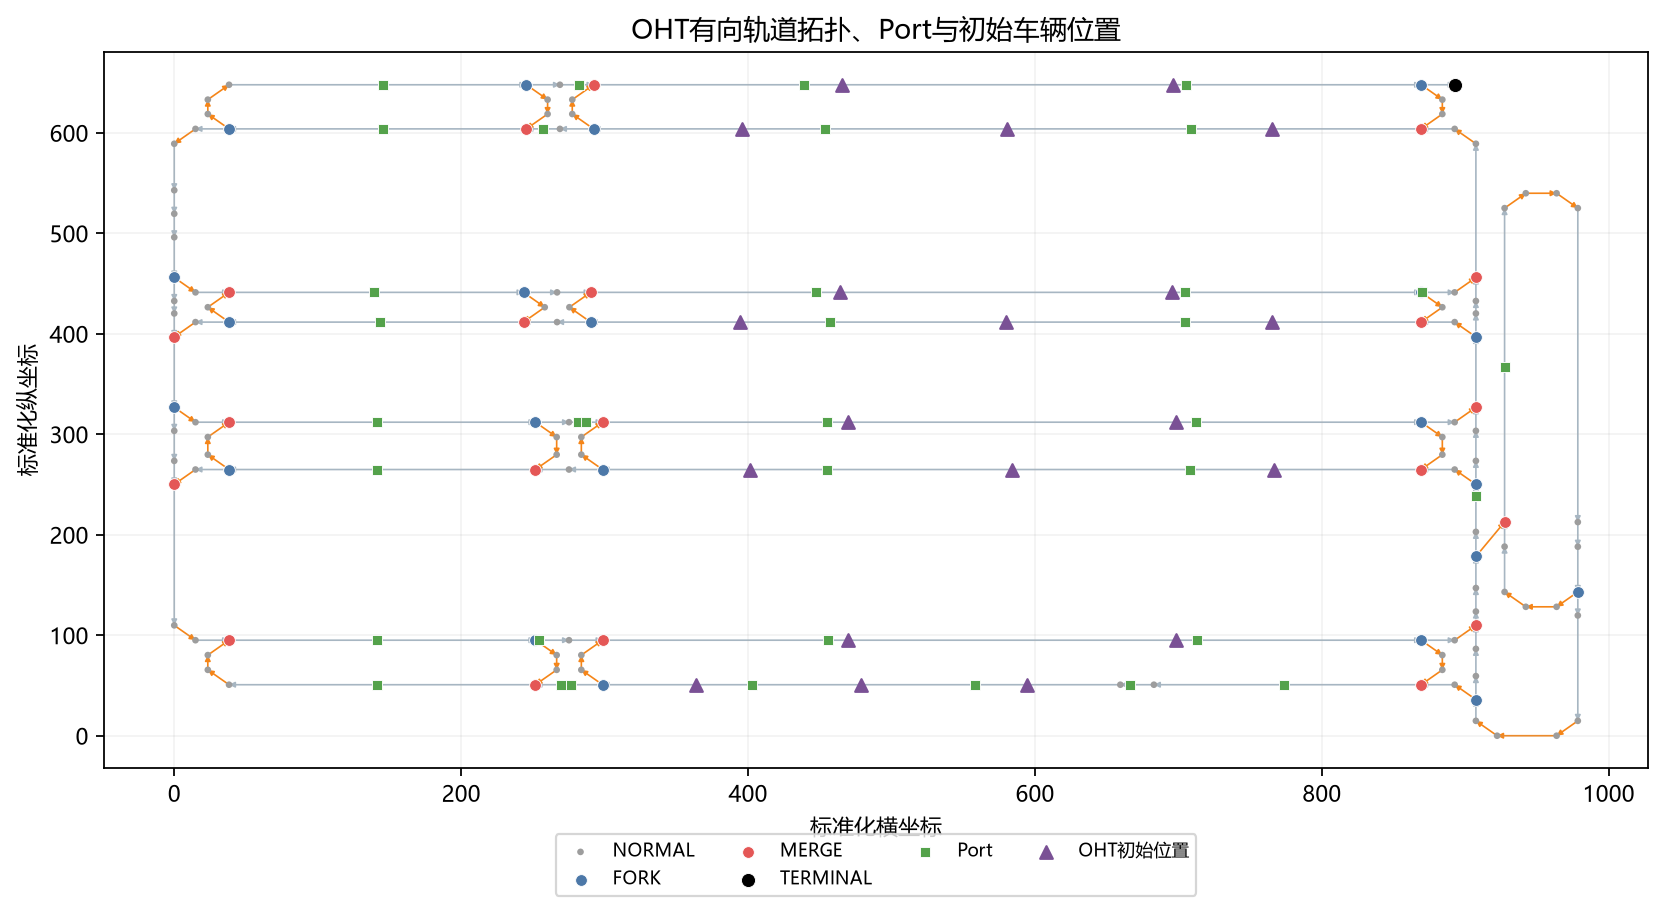
\includegraphics[width=0.98\textwidth]{network_topology.png}
\caption{OHT 有向轨道拓扑、Port 与初始车辆位置}
\label{fig:network-topology}
\end{figure}

对 Link $e$ 上偏移为 $s$ 的位置记为 $(e,s)$，目标 Port 位于 Link $e_p$、偏移 $s_p$。若 $e=e_p$ 且 $s\le s_p$，距离为 $s_p-s$；否则
\begin{equation}\label{eq:position-distance}
D((e,s),p)=L_e-s+\min_{\pi\in\Path(\mathrm{to}(e),\mathrm{from}(e_p))}\sum_{a\in\pi}L_a+s_p.
\end{equation}
式\eqref{eq:position-distance}可按人工手算分为三段。第一段 $L_e-s$ 是车辆从当前位置行至当前 Link 末端的剩余距离；第二段是从当前 Link 下游节点到目标 Link 上游节点的有向最短路；第三段 $s_p$ 是进入目标 Link 后到 Port 的距离。于是完整位置感知距离可写成分段形式
\begin{equation}\label{eq:position-distance-case}
D((e,s),p)=
\begin{cases}
s_p-s, & e=e_p,\ s\le s_p,\\
(L_e-s)+D_V(\mathrm{to}(e),\mathrm{from}(e_p))+s_p,&\text{其他情形},
\end{cases}
\end{equation}
其中 $D_V(u,v)$ 表示节点 $u$ 到 $v$ 的有向最短路长度，范围为 $[0,+\infty]$；若为 $+\infty$，说明该 Port 在当前方向上不可达。特别地，当 $e=e_p$ 且 $s>s_p$ 时，目标虽然在几何上位于车辆后方，但车辆不能逆行，只能先驶出当前 Link，再经有向回路重新进入目标 Link。该分段公式避免使用 $|s_p-s|$ 所造成的“同 Link 逆行捷径”。

对候选路径 $\pi=(e_1,\ldots,e_m)$，自由流时间逐段化简为
\begin{equation}\label{eq:free-flow-time}
\widehat\tau(\pi)=\sum_{q=1}^{m}\frac{\ell_q}{\min\{\bar v_{e_q},v_c\}},
\end{equation}
其中 $\ell_q$ 是路径在 Link $e_q$ 上实际经过的长度，首尾 Link 需扣除起终偏移；$\bar v_{e_q}$ 是附件限速，$v_c=710\ \mathrm{mm/s}$ 是控制巡航上限。式\eqref{eq:free-flow-time}只给出无排队情况下的时间下界，实际时间还要加入取放货、跟驰、资源等待和 Carrier 解锁延迟。

\subsection{任务与互斥资源约束}
\begin{equation}\label{eq:assign-once}
\sum_{k\in K}x_{jk}=1,\qquad j\in J.
\end{equation}
若 $i\prec_c j$ 表示同一 Carrier 的前后继，则
\begin{equation}\label{eq:carrier}
C_i\le A_j,\qquad C_i\le B_j-8.
\end{equation}
对任一 Port、MERGE 或 CurveGroup 资源 $r\in\Res$，
\begin{equation}\label{eq:resource-cap}
\sum_{k\in K}h_{kr}(t)\le1,\qquad \forall t.
\end{equation}
式\eqref{eq:assign-once}保证每项任务恰由一辆车完成，$x_{jk}$ 不允许分数取值，因为一次晶圆载具不能被两辆车分段接力。式\eqref{eq:carrier}中第一项要求后继任务分配不得早于前序放货完成，第二项等价地保证后继取货开始时刻 $B_j-8$ 不早于 $C_i$。两式同时保留是为了分别约束调度提交与物理服务阶段。

对每个资源 $r$ 定义车辆占用时间区间 $I_{kr}=[t_{kr}^{in},t_{kr}^{out})$。Port 的进入时刻为车辆停稳并开始服务的时刻，退出时刻为 $8\ \mathrm{s}$ 服务结束并重新起步的时刻；MERGE 的进入时刻为车头越过停止线的时刻，退出时刻为车尾完全进入唯一确定的下游 Link 的时刻；CurveGroup 的进入时刻为车头进入该组首条 Link 的时刻，退出时刻为车尾离开该组末条 Link 的时刻。因此
\begin{equation}\label{eq:resource-interval}
h_{kr}(t)=\mathbb I\{t\in I_{kr}\},\qquad
I_{kr}\cap I_{\ell r}=\varnothing\quad(k\ne\ell),
\end{equation}
与式\eqref{eq:resource-cap}等价。半开区间使“前车恰好退出、后车同时进入”不会被重复计数。CurveGroup 必须等车尾离开后释放，否则长度为 $950\ \mathrm{mm}$ 的车身仍可能横跨共享弯轨边界；MERGE 未获权车辆则必须在上游满足式\eqref{eq:stop-speed}的可制动位置停车。

\subsection{净空化简与制动速度上界}

轨迹文件记录车辆参考点而非车头、车尾坐标。设前车为 $f$、后车为 $k$，两车长度均为 $L_v$，参考点采用同一车体基准，则前后车参考点的有向距离为 $d_{kf}^{ref}(t)$。前车车尾比其参考点向后偏移一个固定量，后车车头比其参考点向前偏移互补的固定量，两偏移之和正好为车长，因此车身净空可直接化简为
\begin{equation}
g_{kf}(t)=d_{kf}^{ref}(t)-L_v.
\end{equation}
将 $L_v=950\ \mathrm{mm}$ 与题设 $g_0=300\ \mathrm{mm}$ 代入，逐步移项得到
\begin{align}
g_{kf}(t)&\ge g_0,\\
d_{kf}^{ref}(t)-950&\ge300,\\
d_{kf}^{ref}(t)&\ge950+300=1250\ \mathrm{mm}.
\end{align}
故等价硬约束为
\begin{equation}\label{eq:reference-gap}
d_{kf}^{ref}(t)\ge950+300=1250\ \mathrm{mm}.
\end{equation}
为吸收浮点计算、跨 Link 累计和分段重建的数值误差，正式控制器不直接贴近 $1250\ \mathrm{mm}$ 运行，而加 $25\ \mathrm{mm}$ 裕量，取
\begin{equation}\label{eq:control-gap}
d_{ctrl}=1275\ \mathrm{mm}.
\end{equation}

下面推导跟驰速度上界。若车辆以初速度 $v$、恒减速度 $D_{max}$ 制动，利用运动学关系 $v_{end}^2-v^2=2(-D_{max})s$，令末速度 $v_{end}=0$，则停车距离为
\begin{equation}\label{eq:braking-distance}
s_b(v)=\frac{v^2}{2D_{max}}.
\end{equation}
设当前前车速度为 $v_f$、后车速度为 $v_k$。最保守情形是两车同时最大制动，且后车停车点不能越过“前车停车点减去控制间距”的位置。用当前后车参考点作为原点，前车当前参考点位于 $d_{kf}^{ref}$ 处，故停车位置约束为
\begin{equation}
\frac{v_k^2}{2D_{max}}+d_{ctrl}\le d_{kf}^{ref}+\frac{v_f^2}{2D_{max}},
\end{equation}
两边同乘正数 $2D_{max}$，再把与 $v_k$ 无关的项移到右侧，得到
\begin{align}
v_k^2+2D_{max}d_{ctrl}&\le2D_{max}d_{kf}^{ref}+v_f^2,\\
v_k^2&\le v_f^2+2D_{max}(d_{kf}^{ref}-d_{ctrl}).
\end{align}
速度非负，因此开平方后得到跟驰安全速度上界
\begin{equation}\label{eq:safe-speed}
v_k^{follow}\le\sqrt{\max\{0,v_f^2+2D_{max}(d_{kf}^{ref}-d_{ctrl})\}}.
\end{equation}
式中 $v_f,v_k\in[0,710]\ \mathrm{mm/s}$，$d_{kf}^{ref}\ge1250\ \mathrm{mm}$。当根号内为负时，说明后车当前状态已无法仅靠常规制动保留控制裕量，故用 $\max\{0,\cdot\}$ 将命令速度置零并触发硬约束审计。若前方为 Port、MERGE 停止线或任务终点，剩余可用制动距离为 $d_b\ge0$，将式\eqref{eq:braking-distance}改写为 $v^2/(2D_{max})\le d_b$，即
\begin{equation}\label{eq:stop-speed}
v_k^{stop}\le\sqrt{2D_{max}d_b}.
\end{equation}
综合 Link 限速、保守巡航上限 $v_c=710\ \mathrm{mm/s}$、跟驰和停止线四个上界，控制命令取最小值
\begin{equation}
v_k^{cmd}=\min\{\bar v_{e_k},710,v_k^{follow},v_k^{stop}\}.
\end{equation}
这里取最小值的物理意义是：只有同时满足四项限制的速度才可执行。随后以 $\Delta t=0.2\ \mathrm{s}$ 更新。先计算在一步内恰好达到命令速度所需的平均加速度，再裁剪到题设范围：
\begin{align}
a_k(t)&=\operatorname{clip}\left(\frac{v_k^{cmd}-v_k(t)}{\Delta t},-3000,2000\right),\\
v_k(t+\Delta t)&=\max\{0,v_k(t)+a_k(t)\Delta t\},\\
s_k(t+\Delta t)&=s_k(t)+\frac{v_k(t)+v_k(t+\Delta t)}2\Delta t.
\end{align}
第三式并非经验公式。由一步内常加速度 $v(\tau)=v_k(t)+a_k(t)\tau$ 积分可得
\begin{align}
\Delta s&=\int_0^{\Delta t}\left[v_k(t)+a_k(t)\tau\right]d\tau\\
&=v_k(t)\Delta t+\frac12a_k(t)\Delta t^2\\
&=\frac{v_k(t)+v_k(t+\Delta t)}2\Delta t,
\end{align}
即梯形积分在常加速度段上是精确的。若车辆在步内提前停稳，停车时刻 $\tau_s=v_k(t)/D_{max}<\Delta t$，则位移改为
\begin{equation}\label{eq:within-step-stop}
\Delta s=v_k(t)\tau_s-\frac12D_{max}\tau_s^2
=\frac{v_k(t)^2}{2D_{max}},
\end{equation}
余下 $\Delta t-\tau_s$ 时间保持静止。该分段积分禁止“先按整步位移前进、再把末速度截为零”的瞬时停车误差。

\subsection{安全速度的手算工况示例}

为说明式\eqref{eq:safe-speed}如何实际限制车辆，考虑前车已经停稳、两车参考点距离为 $1300\ \mathrm{mm}$ 的紧跟驰工况。代入 $v_f=0$、$D_{max}=3000\ \mathrm{mm/s^2}$、$d_{ctrl}=1275\ \mathrm{mm}$，有
\begin{align}
v_k^{follow}
&\le\sqrt{0^2+2\times3000\times(1300-1275)}\\
&=\sqrt{150000}=387.298\ \mathrm{mm/s}.
\end{align}
故即使当前 Link 限速为 $1000\ \mathrm{mm/s}$，后车命令速度也不得超过 $387.298\ \mathrm{mm/s}$。若参考点距离缩小到 $1275\ \mathrm{mm}$，同样代入可得 $v_k^{follow}=0$，后车必须停车；若距离小于 $1275\ \mathrm{mm}$，根号内可能为负，$\max\{0,\cdot\}$ 仍将命令速度置零，同时审计器记录控制裕量被侵入。

再考虑前方停止线距离 $d_b=50\ \mathrm{mm}$，由式\eqref{eq:stop-speed}
\begin{equation}
v_k^{stop}\le\sqrt{2\times3000\times50}
=547.723\ \mathrm{mm/s}.
\end{equation}
若此时跟驰上界为 $650\ \mathrm{mm/s}$、Link 限速为 $1000\ \mathrm{mm/s}$，则
\begin{equation}
v_k^{cmd}=\min\{1000,710,650,547.723\}
=547.723\ \mathrm{mm/s}.
\end{equation}
这一步展示了各约束不是加权平均，而是由最紧的物理上界直接决定。上述命令速度以最大减速度制动时，停车距离恰为 $50\ \mathrm{mm}$，故不会越过停止线。

对于问题三被淘汰候选，独立回放捕捉到最小参考点距离 $1248\ \mathrm{mm}$。按净空换算式直接手算
\begin{equation}
g_{min}=1248-950=298\ \mathrm{mm}<300\ \mathrm{mm}.
\end{equation}
虽然仅差 $2\ \mathrm{mm}$，仍是明确的硬约束违反，不能用平均时间更小或数值误差解释；因为正式安全裕量本应是正的 $25\ \mathrm{mm}$，而该候选已经越过题设边界。

\subsection{步内连续净空验证}

对每个运动子段，相对参考距离为
\begin{equation}
d(\tau)=d(0)+(v_f-v_k)\tau+\frac12(a_f-a_k)\tau^2.
\end{equation}
令 $\Delta v=v_f-v_k$、$\Delta a=a_f-a_k$，则导数为 $d'(\tau)=\Delta v+\Delta a\tau$。二次函数在闭区间上的极小值只可能出现在端点或合法驻点
\begin{equation}
\tau^*=-\frac{v_f-v_k}{a_f-a_k},\qquad 0<\tau^*<\Delta t.
\end{equation}
因此单个共同运动区间 $[0,\delta]$ 的连续最小距离可人工分三种情况计算：
\begin{equation}\label{eq:continuous-min-case}
d_{min}=
\begin{cases}
\min\{d(0),d(\delta),d(\tau^*)\},&\Delta a\ne0,\ 0<\tau^*<\delta,\\
\min\{d(0),d(\delta)\},&\Delta a\ne0,\ \tau^*\notin(0,\delta),\\
\min\{d(0),d(\delta)\},&\Delta a=0.
\end{cases}
\end{equation}
当 $\Delta a=0$ 时相对距离退化为线性函数，故端点检查已经充分；当 $\Delta a\ne0$ 时只有驻点落入区间才需增加一次代入。验证器先合并两车的加速、制动、静止、越过 Link 端点等全部分段时刻，再在每个共同子区间应用式\eqref{eq:continuous-min-case}。跨 Link 时沿车辆实际计划路径累计有向距离，从而覆盖同 Link、相邻短 Link、MERGE 切入及 CurveGroup 出口形成的新跟驰关系。

与只检查 $t,t+\Delta t$ 两端相比，式\eqref{eq:continuous-min-case}能够识别“步首、步末均安全，但步中先接近后分离”的漏检情形。这也是问题三三个候选虽具有更小平均时间、却因 $298\ \mathrm{mm}$ 步内净空而必须淘汰的判据基础。

\subsection{分层求解的规模化简}

若采用全时间索引 MILP，令 $u_{ket}=1$ 表示车辆 $k$ 在步 $t$ 占用 Link $e$，仅该类变量数量就是
\begin{equation}
|K||E|\frac{T_H}{\Delta t}=20\times152\times\frac{7200}{0.2}
=109{,}440{,}000.
\end{equation}
若再为 90 个互斥资源设置占用变量，至少还需
\begin{equation}
20\times90\times36{,}000=64{,}800{,}000
\end{equation}
个二元状态，尚未计入任务顺序、路径选择和成对净空约束。成对车辆--时间约束的数量级为
\begin{equation}
\binom{20}{2}\times36{,}000=6{,}840{,}000,
\end{equation}
且其中还包含非线性运动学或大量 Big-$M$ 线性化。故完整模型远超竞赛实时求解预算。

本文把组合决策限制在任务链、候选路径和队列插入位置上；一旦上层给出承诺队列，下层直接按 $0.2\ \mathrm{s}$ 步长执行确定性资源仲裁与运动控制。这样，上层候选的规模主要随 $|J||K|\bar q$ 增长，而非随 $|K||E|T_H/\Delta t$ 增长。该化简不删除任何物理硬约束，而是把硬约束从巨型优化模型转移到统一可复核的仿真内核中。

\section{问题一：静态任务分配与协同运行}
\subsection{模型选择理由}

问题一同时决定 32 项任务的车辆归属、20 条车内任务链以及每一段空载/载货路径，本质上是带资源约束的多车辆取送路径问题（PDVRP-RC）。精确 MILP 能给出较强最优性结论，但显式加入 $0.2\ \mathrm{s}$ 运动和冲突资源后规模过大；遗传算法编码简单，但任务移除后对车辆链的局部修复能力较弱。ALNS 可通过多种破坏算子跳出局部最优，又能用 regret 插入快速恢复任务链，适合“任务规模有限、真实评价昂贵、约束复杂”的取送问题\cite{ropke2006,shaw1998}。因此本文用代理成本 ALNS 搜索任务链，再用高保真仿真评价正式指标。

\subsection{静态 PDVRP-RC 模型}

定义 $y_{ij}^{k}=1$ 表示车辆 $k$ 在任务 $i$ 后紧接执行任务 $j$，虚拟任务 $0_k$ 表示车辆初始位置。除式\eqref{eq:assign-once}外，车辆链满足
\begin{align}
\sum_i y_{ij}^{k}&=x_{jk},\qquad \forall j,k,\\
\sum_j y_{ij}^{k}&=x_{ik},\qquad \forall i,k.
\end{align}
第一式表示被车辆 $k$ 执行的任务 $j$ 恰有一个直接前驱，第二式表示任务 $i$ 恰有一个直接后继；车辆链的最后一个任务连接虚拟终点，故不会形成孤立子链。为便于写出取放货先后关系，定义 $S_j=B_j-8$ 为取货开始时刻，$F_j=C_j-8$ 为放货开始时刻。于是单任务内部顺序为
\begin{align}
A_j&\le S_j,\\
B_j&=S_j+8,\\
F_j&\ge B_j+\tau_j^{load},\\
C_j&=F_j+8,
\end{align}
其中 $\tau_j^{load}\ge0$ 为由式\eqref{eq:free-flow-time}估计的载货自由流下界；正式仿真中 $F_j-B_j$ 还包含跟驰、资源等待和速度调整。任务执行时间可逐项分解为
\begin{align}\label{eq:transfer-decomposition}
C_j-r_j={}&(A_j-r_j)+(S_j-A_j)+8\\
&+\tau_j^{load}+W_j^{traffic}+\delta_j^{ctrl}+8,
\end{align}
右侧依次为分配等待、分配后取货等待、取货服务、自由流下界、停车等待、非停车速度调整损失和放货服务。其中载货阶段满足
\begin{equation}
F_j-B_j=\tau_j^{load}+W_j^{traffic}+\delta_j^{ctrl}.
\end{equation}
正式输出中的平均分配、取货响应、载货运输和暂停时间均由该时间轴复算，而非彼此独立估计。

若 $y_{ij}^{k}=1$，则任务时序满足 $A_j\ge C_i+\tau_{ij}^{empty}$；若 $y_{ij}^{k}=0$，该约束应失效。采用 Big-$M$ 写成
\begin{equation}\label{eq:bigm-sequence}
A_j\ge C_i+\tau_{ij}^{empty}-M(1-y_{ij}^{k}).
\end{equation}
当 $y_{ij}^{k}=1$ 时，右侧最后一项为 0，恢复真实先后约束；当 $y_{ij}^{k}=0$ 时，取 $M=T_H+\max\tau_{ij}^{empty}$，右侧降至非约束水平。$\tau_{ij}^{empty}$ 是任务 $i$ 的目的 Port 到任务 $j$ 源 Port 的空载耗时，其代理值由式\eqref{eq:free-flow-time}计算，正式值由仿真产生。

每个 OD 对预生成至多 $R=3$ 条无环有向候选路径。令 $z_{j\rho}^{L}$ 和 $z_{j\rho}^{E}$ 分别表示任务 $j$ 的载货段、其前置空载段是否选择第 $\rho$ 条候选路径，则
\begin{equation}\label{eq:path-choice}
\sum_{\rho=1}^{R}z_{j\rho}^{L}=1,\qquad
\sum_{\rho=1}^{R}z_{j\rho}^{E}=1,
\end{equation}
且只有在路径可达时变量才被创建。路径候选按“自由流时间+资源惩罚”排序，既保留最短路，也允许搜索绕开高冲突 MERGE 和 CurveGroup。

问题一全部任务在 $r_j=0$ 时释放，故正式目标为
\begin{equation}
\min \bar T=\frac1{32}\sum_{j=1}^{32}C_j.
\end{equation}
由于每个候选都运行完整仿真代价较高，搜索阶段采用代理目标
\begin{equation}\label{eq:q1-surrogate}
\widetilde F=\sum_j\widehat C_j+\eta_1\widehat T_{\max}+\eta_2D^{empty}+\eta_3\sum_j w(p_j)\widehat C_j.
\end{equation}
其中 $\widehat C_j$ 基于位置感知自由流路径估计。式\eqref{eq:q1-surrogate}只用于候选排序；最终一定按完整仿真的 $\bar T$ 选择，避免代理误差改变题目目标。

代理目标中，$\sum_j\widehat C_j$ 对应官方平均时间的常数倍；$\widehat T_{\max}$ 防止少数车辆队列过长；$D^{empty}$ 降低无效空驶；$w(p_j)\widehat C_j$ 对高优先级任务施加附加拖期成本。四项量纲分别为 s、s、mm 和 s，因此 $\eta_2$ 的单位为 s/mm，其余权重无量纲。所有权重只在代理层生效，正式比较仍完全采用式\eqref{eq:official-objective}和硬门结果。

\subsection{ALNS 求解过程}

先用全局最小增量插入构造初解，再固定随机种子 20260815 运行 1200 轮 ALNS。破坏算子包括随机移除、最差边际贡献移除和相关任务移除，修复采用 regret-3 插入；候选用模拟退火准则接受\cite{kirkpatrick1983}。流程见图\ref{fig:alns-flow}。
\begin{figure}[H]
\centering
\begin{tikzpicture}[node distance=0.55cm]
\node[flow] (init) {全局最小增量插入构造初解};
\node[flow,below=of init] (destroy) {自适应选择破坏算子并移除任务};
\node[flow,below=of destroy,fill=flowgreen] (repair) {regret-3 插入修复 20 条车辆链};
\node[flow,below=of repair] (evaluate) {计算代理目标 $\widetilde F$};
\node[decision,below=0.8cm of evaluate] (accept) {接受候选？};
\node[flow,below left=0.72cm and 1.45cm of accept,fill=flowgray] (retain) {保留当前解};
\node[flow,below right=0.72cm and 1.45cm of accept,fill=flowgreen] (update) {更新当前解/历史最优};
\node[decision,below=2.1cm of accept] (stop) {达到 1200 轮？};
\node[flow,below=0.72cm of stop,fill=floworange] (sim) {最好任务链进入完整物理仿真};
\draw[arrow] (init)--(destroy); \draw[arrow] (destroy)--(repair); \draw[arrow] (repair)--(evaluate); \draw[arrow] (evaluate)--(accept);
\draw[arrow] (accept)--node[above left,font=\small]{否}(retain); \draw[arrow] (accept)--node[above right,font=\small]{是}(update);
\draw[arrow] (retain)--(stop); \draw[arrow] (update)--(stop); \draw[arrow] (stop)--node[right,font=\small]{是}(sim);
\draw[arrow] (stop.west) -| ++(-2.5,0) |- node[pos=0.25,left,font=\small]{否}(destroy.west);
\end{tikzpicture}
\caption{问题一 ALNS 静态调度流程}
\label{fig:alns-flow}
\end{figure}

具体地，设当前解为 $s$，删除任务 $j$ 后的代理目标为 $\widetilde F(s\setminus j)$，则最差贡献分数定义为
\begin{equation}\label{eq:worst-removal}
\Delta_j^{remove}=\widetilde F(s)-\widetilde F(s\setminus j).
\end{equation}
$\Delta_j^{remove}$ 越大，说明任务 $j$ 在当前位置造成的边际成本越高，优先移除更可能得到改进。相关移除则根据 Source、Destination、释放时刻和 Carrier 相似性定义
\begin{equation}\label{eq:relatedness}
R_{ij}=\alpha_d\frac{D(S_i,S_j)+D(D_i,D_j)}{D_{max}^{net}}
+\alpha_p\frac{|p_i-p_j|}{p_{max}-p_{min}}
+\alpha_c\mathbb I(c_i\ne c_j),
\end{equation}
其中各比例项均归一化到 $[0,1]$，$R_{ij}$ 越小表示两任务越相关；成组移除它们可以重新组织同一区域的任务链。

修复阶段对未插入任务 $j$ 枚举所有车辆、位置和路径，得到从小到大排列的前三个插入增量 $\Delta_j^{(1)}\le\Delta_j^{(2)}\le\Delta_j^{(3)}$。regret-3 值为
\begin{equation}\label{eq:regret3}
\operatorname{Regret}_3(j)=
(\Delta_j^{(2)}-\Delta_j^{(1)})+(\Delta_j^{(3)}-\Delta_j^{(1)}).
\end{equation}
若该值很大，说明错过最佳插入位置后成本会显著上升，因此应先固定该任务。每次选择 regret-3 最大的任务，并采用其最佳插入位置，直至所有被移除任务重新进入车辆链。

设候选解为 $s'$、代理目标差为 $\Delta F=\widetilde F(s')-\widetilde F(s)$。若 $\Delta F\le0$ 则必然接受；否则按模拟退火概率
\begin{equation}\label{eq:sa-accept}
P_{acc}=\exp\left(-\frac{\Delta F}{T_n}\right),\qquad
T_{n+1}=\gamma T_n,quad0<\gamma<1
\end{equation}
接受。初期温度较高，可跨越局部最优；后期温度降低，搜索逐渐稳定。每经过一个评分周期，根据算子获得“刷新全局最好、改善当前解、被接受、被拒绝”四类得分更新权重
\begin{equation}\label{eq:operator-weight}
\omega_m^{new}=(1-\rho)\omega_m^{old}
+\rho\frac{\mathrm{score}_m}{\max\{1,\mathrm{use}_m\}},
\end{equation}
其中 $\rho\in(0,1)$ 是记忆更新率。这样，近期有效的破坏/修复算子被更频繁选择，但所有算子仍保留非零概率。

1200 轮中接受 1119 个候选，历史最好代理解改进 46 次。最终 8 辆 OHT 执行 1 项任务，12 辆执行 2 项任务，20 辆车均被使用。车辆工作量分布见图\ref{fig:q1-workload}，其信息价值在于说明平均时间的降低并非依靠少数车辆超负荷，而是来自较均匀的任务链重组。

\begin{figure}[H]
\centering
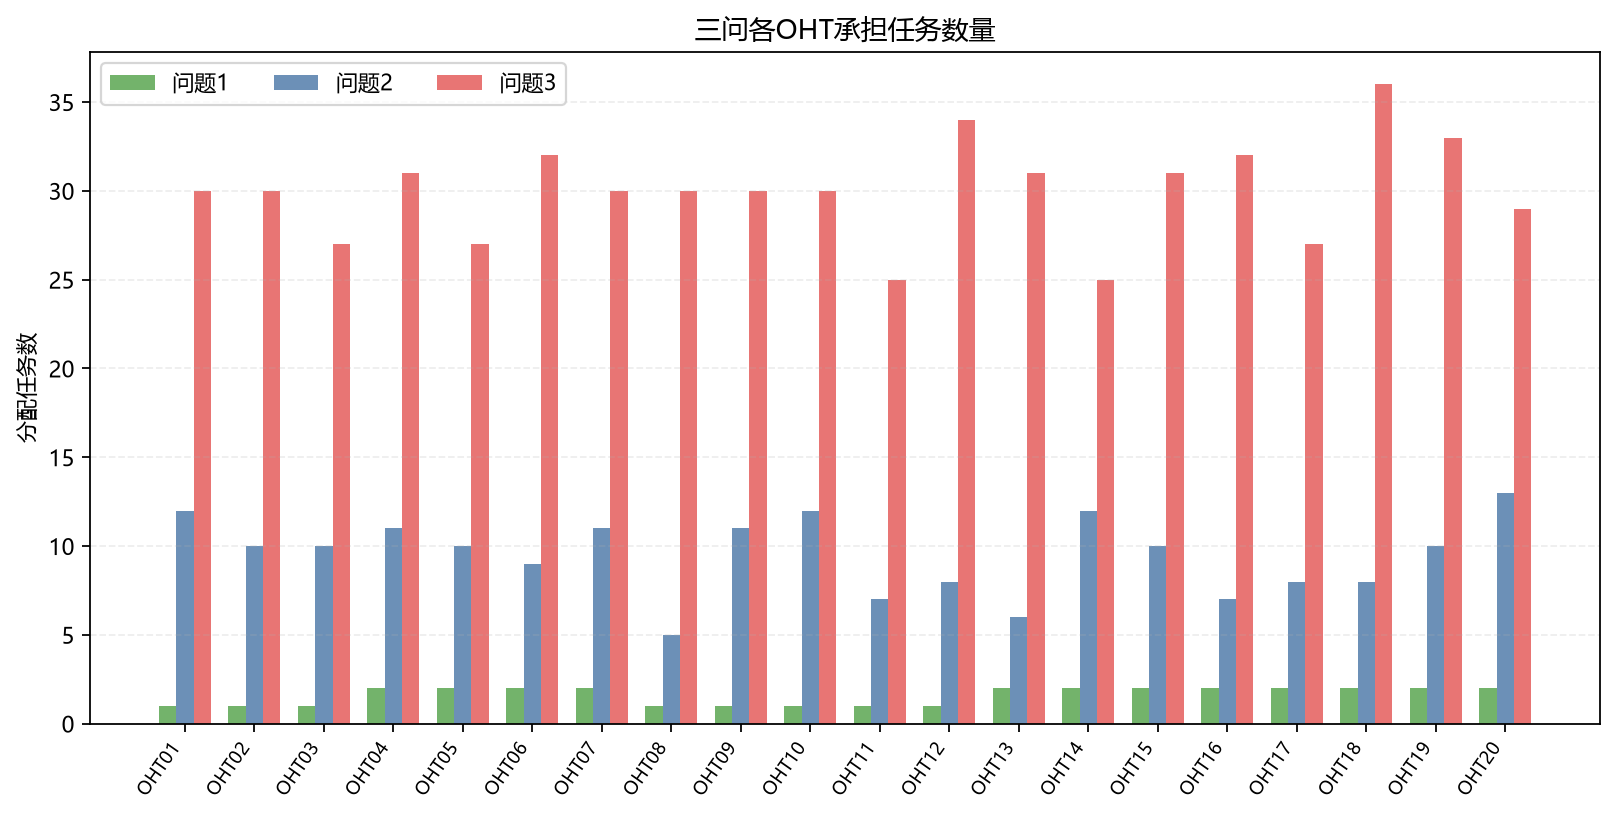
\includegraphics[width=0.82\textwidth]{vehicle_workload.png}
\caption{问题一 ALNS 方案的车辆任务量分布}
\label{fig:q1-workload}
\end{figure}

\begin{table}[H]
\centering
\caption{问题一候选优化方法的适用性比较}
\label{tab:q1-method-choice}
\renewcommand{\arraystretch}{1.28}
\begin{tabular*}{\textwidth}{@{\extracolsep{\fill}}p{2.4cm}p{3.4cm}p{3.5cm}p{4.1cm}@{}}
\toprule[1pt]
方法 & 主要优势 & 主要局限 & 本题选择结论\\ \midrule
全时域 MILP & 可在小规模下给出最优性界；约束表达统一 & 时间索引变量超过亿级，连续净空需大量线性化 & 适合小规模离线基准，不适合本题完整物理时域\\
遗传算法 & 编码直观、全局探索能力较强，易并行 & 交叉后易破坏任务链与 Carrier 顺序，可行修复成本高 & 可作备选，但对“删除--局部修复”结构利用不足\\
ALNS & 破坏尺度可变，regret 插入擅长修复任务链，可接高代价仿真 & 不提供全局最优证明，需设置迭代预算 & 与 PDVRP-RC 结构吻合，作为正式静态求解器\\
\bottomrule[1pt]
\end{tabular*}
\end{table}

\subsection{算法比较与结果}
\begin{table}[H]
\centering
\caption{问题一三种静态调度方案比较}
\renewcommand{\arraystretch}{1.35}
\begin{tabular*}{\textwidth}{@{\extracolsep{\fill}}lcccc@{}}
\toprule[1pt]
方案 & 平均任务执行时间/s & Makespan/s & 完成任务 & 硬违规\\ \midrule
基准追加调度 & 206.51875 & 406.0 & 32 & 0\\
全局增量插入 & 193.16875 & 401.6 & 32 & 0\\
ALNS 静态调度 & \textbf{171.39375} & \textbf{332.8} & 32 & 0\\
\bottomrule[1pt]
\end{tabular*}
\label{tab:q1-compare}
\end{table}

\begin{figure}[H]
\centering
\begin{tikzpicture}
\begin{axis}[ybar,width=0.82\textwidth,height=6.0cm,ymin=0,ymax=230,ylabel={平均任务执行时间/s},symbolic x coords={基准追加,增量插入,ALNS},xtick=data,nodes near coords,bar width=22pt,grid=major,grid style={dashed,gray!30}]
\addplot[fill=blue!45] coordinates {(基准追加,206.51875) (增量插入,193.16875) (ALNS,171.39375)};
\end{axis}
\end{tikzpicture}
\caption{问题一静态调度平均任务执行时间对比}
\end{figure}

ALNS 相较基准降低 $17.01\%$，相较增量插入进一步降低 $11.27\%$。正式指标为：平均取货响应时间 $67.331250\ \mathrm{s}$、平均载货运输时间 $88.062500\ \mathrm{s}$、平均暂停时间 $1.381250\ \mathrm{s}$、平均空载距离 $18014.268750\ \mathrm{mm}$、平均总距离 $79285.559375\ \mathrm{mm}$。

图\ref{fig:time-distribution}左侧箱线图进一步表明，问题一任务执行时间主要集中在较低区间，并未因优化均值而产生极端长尾；问题三则出现显著更宽的四分位距和约 $3000\ \mathrm{s}$ 的长尾。右侧经验分布用于后文比较动态场景的完成节奏。

\begin{figure}[H]
\centering
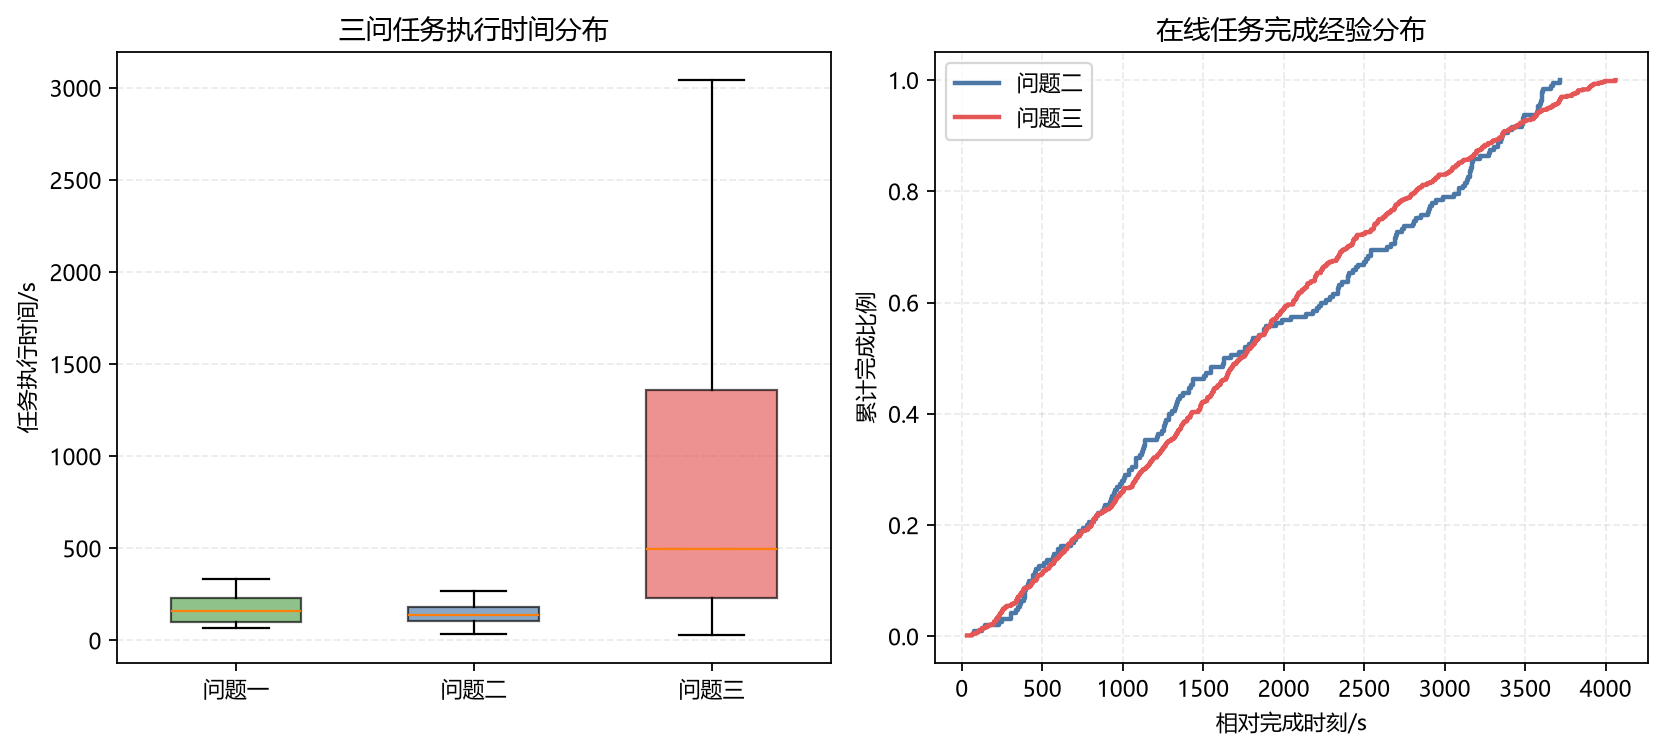
\includegraphics[width=0.98\textwidth]{time_distribution_and_completion.png}
\caption{三问任务执行时间箱线图与在线任务完成经验分布}
\label{fig:time-distribution}
\end{figure}

\section{问题二：190 项动态任务在线调度}
\subsection{在线状态与模型选择}

问题二中未来任务不可见，离线 ALNS 不能直接使用。每次到达后重解大规模 MIP/MPC 会造成较长决策延迟\cite{rawlings2017}；强化学习需要额外训练场景且难以直接保证硬约束\cite{sutton2018}。滚动拍卖把“车辆选择”和“队列插入位置”统一为报价比较，并在每次提交后更新车辆状态，具有计算快、可解释和便于接入当前拥堵信息的优点\cite{bertsekas1988}。

图\ref{fig:arrival-curves}给出问题二、三按首个释放时刻平移后的累计到达曲线。问题二 190 项任务分散在 $3558.816\ \mathrm{s}$ 内到达，曲线斜率较缓；问题三在约 $1797\ \mathrm{s}$ 内释放 600 项任务，曲线持续陡升。两者具有相同路网和车辆数量，却处在完全不同的负载区间，因此在线算法必须根据当前状态决策，而不能预先复制静态任务链。

\begin{figure}[H]
\centering
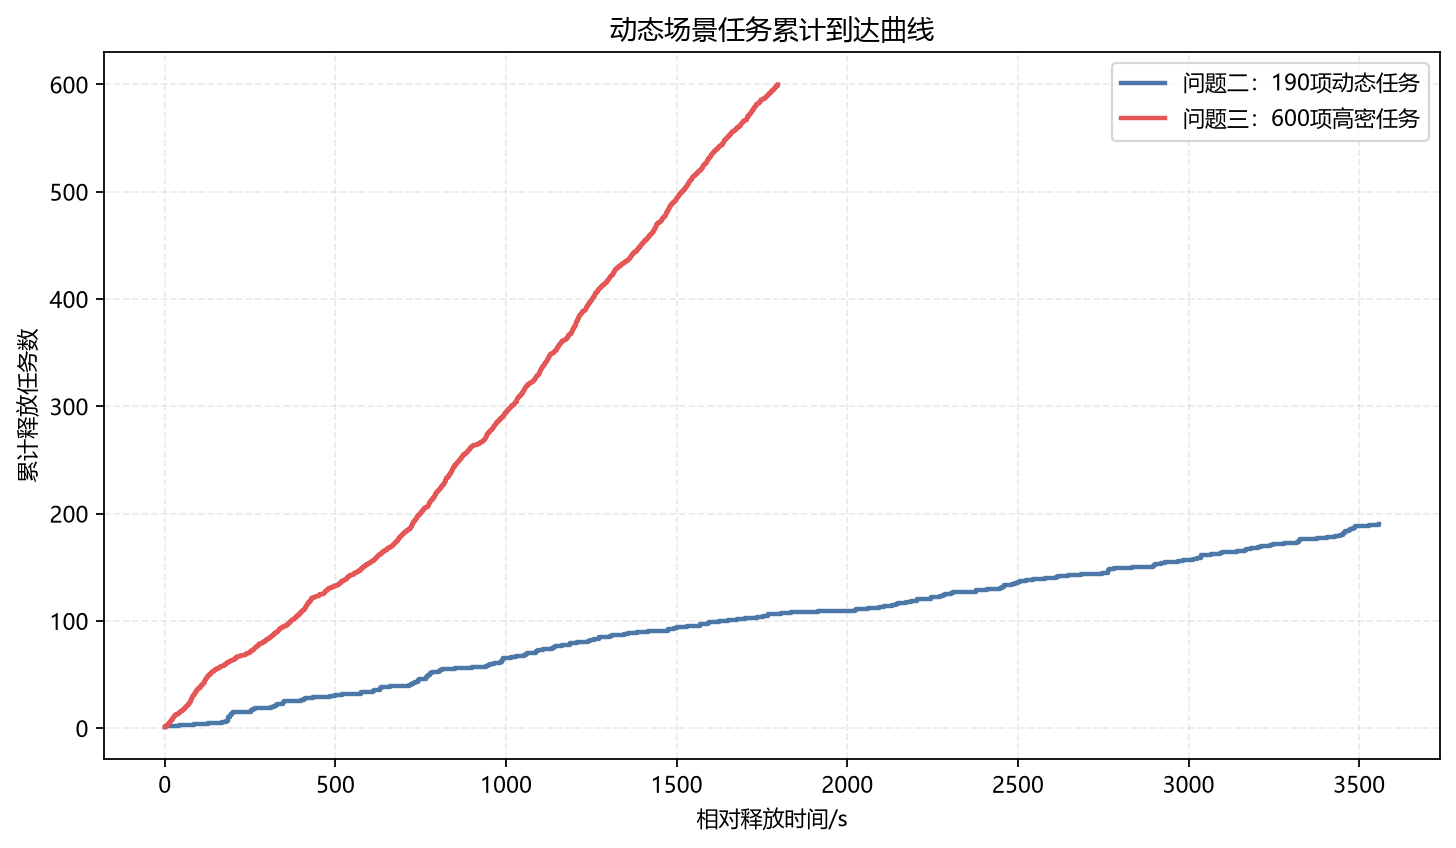
\includegraphics[width=0.88\textwidth]{arrival_curves.png}
\caption{问题二、三动态任务累计到达曲线}
\label{fig:arrival-curves}
\end{figure}

定义时刻 $t$ 已释放且 Carrier 前序完成的可分配集合为 $J^V(t)$，已释放但仍被前序阻塞的集合为 $J^B(t)$。在线状态为
\begin{equation}
S(t)=\{J^V(t),J^B(t),e_k(t),s_k(t),v_k(t),Q_k(t),R(t),H(t)\},
\end{equation}
其中 $R(t)$ 为当前资源占用，$H(t)$ 只包含已经发生的等待与拥堵统计。调度器接口只传入 $J^V(t)$，不传入未来任务字段。

集合的构造可写为
\begin{align}
J^{rel}(t)&=\{j\in J:r_j\le t,\ C_j\text{ 尚未产生}\},\\
J^V(t)&=\{j\in J^{rel}(t):\operatorname{pred}(j)=\varnothing
\ \text{或}\ C_{\operatorname{pred}(j)}\le t\},\\
J^B(t)&=J^{rel}(t)\setminus J^V(t).
\end{align}
其中 $\operatorname{pred}(j)$ 为同一 Carrier 的直接前序任务。每当车辆完成放货，验证器只检查以该任务为直接前序的已释放后继，将满足条件者从 $J^B(t)$ 移入 $J^V(t)$。尚未释放的任务不进入任何在线集合，因此其 Source、Destination、Priority 和 CarrierID 不可能参与报价计算。

\subsection{滚动拍卖报价及化简}

对任务 $j$、车辆 $k$ 和队列插入位置 $q$，报价定义为
\begin{align}\label{eq:q2-bid}
b_{jkq}={}&\widehat C_{jkq}-r_j+\lambda_1\Delta D_{jkq}^{empty}+\lambda_2\Delta W_{jkq}
+\lambda_3\operatorname{CongRisk}_{jkq}\notag\\
&-\lambda_4p_j-\lambda_5\operatorname{Age}_j+\lambda_6\Delta\sum_{h\in Q_k}\widehat C_h.
\end{align}
第一项近似官方主目标；空载、等待和拥堵项抑制队列扩散；优先级和年龄项防止任务饥饿；最后一项限制新任务对既有队列的拖延。由于原始指标同时含 s、mm 和无量纲计数，实现时先采用稳健区间归一化
\begin{equation}\label{eq:robust-normalize}
\mathcal N(x)=\operatorname{clip}\left(
\frac{x-x_{0.05}}{x_{0.95}-x_{0.05}+\varepsilon},0,1\right),
\end{equation}
其中 $x_{0.05},x_{0.95}$ 是当前可见候选的 5\% 和 95\% 分位数，$\varepsilon>0$ 防止分母为零。于是等效时间报价可理解为
\begin{align}\label{eq:q2-bid-normalized}
b_{jkq}={}&(\widehat C_{jkq}-r_j)
+\beta_D\mathcal N(\Delta D_{jkq}^{empty})
+\beta_W\mathcal N(\Delta W_{jkq})\\
&+\beta_G\mathcal N(\operatorname{CongRisk}_{jkq})
-\beta_P\mathcal N(p_j)-\beta_A\mathcal N(t-r_j)
+\beta_Q\mathcal N\!\left(\Delta\sum_{h\in Q_k}\widehat C_h\right),\notag
\end{align}
其中 $\beta_D,\ldots,\beta_Q$ 的单位统一为 s。归一化后每个修正项的绝对影响不超过相应权重，避免大数值的距离项仅因量纲而压倒预计完成时间。

逐项说明如下：$\widehat C_{jkq}-r_j\ge16\ \mathrm{s}$ 是任务在候选插入下的预计执行时间；$\Delta D^{empty}\ge0$ 是因插入任务新增的空载距离；$\Delta W\ge0$ 是车辆队列的预计等待增量；$\operatorname{CongRisk}\ge0$ 统计候选路径上当前已发生的资源排队；优先级 $p_j$ 位于附件给定范围内，数值越大越优先；年龄 $t-r_j\ge0$ 随等待增长；最后一项是对队列中既有任务预计完成时刻总和的增量。这样，报价较小表示对官方目标和既有承诺的综合扰动较小。

考虑到单个触发时刻可见任务数有限，本文用逐项最小报价化简组合指派：每次选择最小的 $(j,k,q)$，提交后更新 $Q_k$ 和剩余报价，直至当前可见集合为空。该方法牺牲单批严格全局最优性，但把决策转化为可实时枚举的小问题，并由后续事件滚动修正。

若当前可见任务数为 $m$、车辆数为 $K=20$、车辆平均承诺队列长度为 $\bar q$、每个 OD 保留 $R$ 条路径，则一轮完整枚举复杂度约为
\begin{equation}
O(mK(\bar q+1)R).
\end{equation}
每提交一项任务后 $m$ 减 1，故单个事件批次的最坏复杂度为 $O(m^2K(\bar q+1)R)$。在问题二中到达较分散，绝大多数触发时刻 $m$ 很小，因而能够在下一控制步前完成决策。

\subsection{事件触发与稳定机制}

算法支持新任务释放、车辆完成、到达 FORK、资源等待超过 $5\ \mathrm{s}$、等待图成环风险和每 $3\ \mathrm{s}$ 心跳六类触发。未取货任务设置 $8\ \mathrm{s}$ 承诺锁定期、$10\ \mathrm{s}$ 冷却期，并要求预测改善超过 $300\ \mathrm{s}$ 才允许重排；已取货任务永久冻结。正式 balanced 轨迹中 190 次决策完成全部任务，没有发生重分配和显式预约，说明本场景下复杂触发机制退化为稳定的一次到达一次决策。

\begin{figure}[H]
\centering
\begin{tikzpicture}[node distance=0.58cm]
\node[data] (event) {新任务/完成/冲突等待/心跳事件};
\node[flow,below=of event] (visible) {更新 $J^V(t)$，解锁 Carrier 后继};
\node[flow,below=of visible,fill=flowgreen] (enum) {枚举车辆与全部合法插入位置};
\node[flow,below=of enum] (bid) {计算式\eqref{eq:q2-bid}报价};
\node[decision,below=0.8cm of bid] (ready) {仍有可分配任务？};
\node[flow,below left=0.75cm and 1.45cm of ready,fill=flowgreen] (commit) {提交最小报价并更新队列};
\node[flow,below right=0.75cm and 1.45cm of ready,fill=floworange] (run) {进入统一交通仿真};
\draw[arrow] (event)--(visible); \draw[arrow] (visible)--(enum); \draw[arrow] (enum)--(bid); \draw[arrow] (bid)--(ready);
\draw[arrow] (ready)--node[above left,font=\small]{是}(commit); \draw[arrow] (commit.west) -| ++(-1,0) |- (enum.west);
\draw[arrow] (ready)--node[above right,font=\small]{否}(run);
\end{tikzpicture}
\caption{问题二事件触发滚动拍卖流程}
\label{fig:q2-flow}
\end{figure}

\begin{table}[H]
\centering
\caption{问题二在线优化方法的选择比较}
\label{tab:q2-method-choice}
\renewcommand{\arraystretch}{1.28}
\begin{tabular*}{\textwidth}{@{\extracolsep{\fill}}p{2.7cm}p{3.3cm}p{3.5cm}p{4.0cm}@{}}
\toprule[1pt]
方法 & 主要优势 & 主要局限 & 本题选择结论\\ \midrule
滚动时域 MILP/MPC & 能显式处理短期预测和多约束，可给局部最优解 & 每次事件均需重建整数模型；未来任务不可见时预测窗口信息有限 & 可用于较慢节拍系统，本题决策频率下计算负担偏大\\
强化学习 & 在线推断速度快，可从大量场景学习非线性策略 & 需要训练分布；难对未见路况解释；安全约束仍需外置屏障 & 缺少训练样本与可认证安全保证，不作为正式方案\\
滚动拍卖 & 只使用当前可见信息，报价可解释，增量更新快 & 单次贪心提交不保证批次全局最优 & 与在线信息约束和实时预算匹配，作为正式算法\\
\bottomrule[1pt]
\end{tabular*}
\end{table}

\subsection{算法比较与正式结果}
\begin{table}[H]
\centering
\caption{问题二在线算法比较}
\renewcommand{\arraystretch}{1.34}
\begin{tabular*}{\textwidth}{@{\extracolsep{\fill}}p{4.7cm}cccc@{}}
\toprule[1pt]
算法 & 平均执行时间/s & Makespan/s & 硬违规 & 未来泄漏\\ \midrule
在线 FCFS & 142.946305 & 3715.2 & 0 & 0\\
滚动最小增量插入 & 142.946305 & 3715.2 & 0 & 0\\
负载均衡滚动拍卖 & \textbf{142.946305} & \textbf{3715.2} & 0 & 0\\
事件触发拍卖--预约完整候选 & 147.716832 & 3721.2 & 0 & 0\\
\bottomrule[1pt]
\end{tabular*}
\label{tab:q2-compare}
\end{table}

前三个方案完全同分，说明任务到达间隔、车辆可用性与最低巡航速度共同使其产生相同实际分配；balanced 仅由预先确定的平局规则选中，不能把同分解释为额外性能增益。完整候选虽生成 4658 条预约事件，但平均执行时间反而增加 $4.770527\ \mathrm{s}$，表明中等负载下过度重规划会引入稳定性成本。

图\ref{fig:candidate-comparisons}左图直观显示前三个问题二候选完全等高，而完整候选较差；右图同时标注问题三候选的平均时间和最小净空，绿色只代表通过 $300\ \mathrm{mm}$ 硬门的直接滚动方案。该图避免只看柱高而误把不安全候选识别为改进方案。

\begin{figure}[H]
\centering
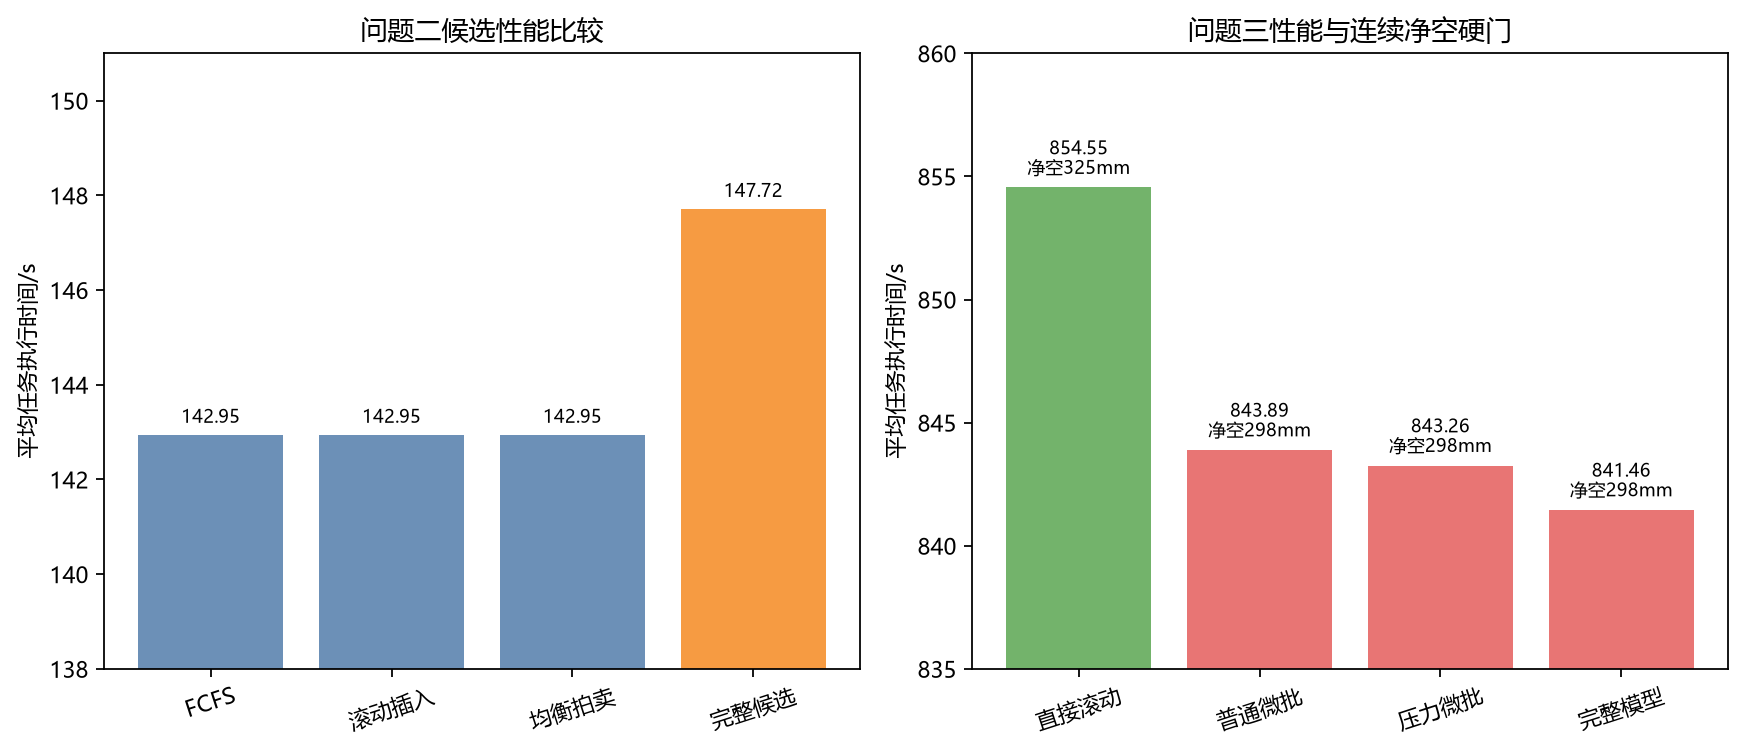
\includegraphics[width=0.98\textwidth]{candidate_comparisons.png}
\caption{问题二候选性能及问题三“性能--安全”联合比较}
\label{fig:candidate-comparisons}
\end{figure}

\begin{sloppypar}
问题二正式方案的平均分配等待为 $1.713674\ \mathrm{s}$，平均取货响应为 $35.904211\ \mathrm{s}$，平均载货运输为 $89.328421\ \mathrm{s}$，平均暂停为 $2.436842\ \mathrm{s}$，平均空载距离为 $22403.424029\ \mathrm{mm}$，平均总距离为 $84672.440345\ \mathrm{mm}$。
\end{sloppypar}

\section{问题三：高负载动态任务协同调度}
\subsection{高密场景特征与正式模型}

问题三在约 $1797\ \mathrm{s}$ 内释放 600 项任务，平均每 $3\ \mathrm{s}$ 到达一项，20 辆 OHT 长时间连续工作。此时延迟不再主要来自单项载货路径，而来自可用车辆不足、Carrier 阻塞、Source 排队与汇流切入。本文仍以问题二的滚动插入作为可行基线，并额外设计普通微批、压力感知微批和“压力+时隙+等待图”完整候选，以检验批处理与显式资源协同是否改善高负载性能。

先对负载强度作手算。以任务释放跨度近似观察窗，问题二、三的平均到达率分别为
\begin{align}
\lambda_2&=\frac{190}{3558.816}=0.0533885\ \mathrm{task/s},\\
\lambda_3&=\frac{600}{1797}=0.3338898\ \mathrm{task/s},\\
\frac{\lambda_3}{\lambda_2}&=6.254.
\end{align}
再构造一个对系统最有利的容量上界：忽略所有空驶、分配等待、Carrier 阻塞和交通暂停，每项任务也至少需要平均载货时间加两次 $8\ \mathrm{s}$ 服务。由正式轨迹的平均载货时间，20 辆车的乐观处理率为
\begin{align}
\mu_2^{upper}&=\frac{20}{89.328421+16}=0.189882\ \mathrm{task/s},\\
\mu_3^{upper}&=\frac{20}{89.227333+16}=0.190065\ \mathrm{task/s}.
\end{align}
问题二满足 $\lambda_2<\mu_2^{upper}$，到达任务原则上可被逐步消化；问题三却有 $\lambda_3>\mu_3^{upper}$，且超载比
\begin{equation}\label{eq:overload-ratio}
\rho_3^{lower}=\frac{\lambda_3}{\mu_3^{upper}}=1.757>1.
\end{equation}
这里称“下界”是因为真实系统还存在空驶和冲突，实际负载率只会更高。故在问题三的集中释放阶段，任何算法都不可能即时完成全部到达任务，队列增长具有结构必然性；算法目标是抑制队列扩散并保证安全，而不是消除不可避免的等待。

定义可行候选集
\begin{equation}\label{eq:feasible-set}
\Omega_F=\{\omega:N_{done}=600,\ V_{hard}(\omega)=0,
g_{min}(\omega)\ge300,\ L_{future}(\omega)=0\},
\end{equation}
并在其中选择
\begin{equation}\label{eq:lex-select}
\omega^*=\argmin_{\omega\in\Omega_F}
\left(\bar T(\omega),T_{\max}(\omega),\operatorname{Name}(\omega)\right).
\end{equation}
式\eqref{eq:feasible-set}将安全、资源、Carrier、运动学和在线性作为硬门；式\eqref{eq:lex-select}才使用官方目标，避免平均时间更小但存在碰撞风险的方案被错误选中。

集合 $\Omega_F$ 中，$N_{done}$ 是仿真终止前完成任务数，范围为 $[0,600]$；$V_{hard}$ 是运动学、资源容量、Carrier、方向与格式违规总数，必须等于 0；$g_{min}$ 是对全部车辆对、全部连续运动子段求得的最小车身净空；$L_{future}$ 是未来信息泄漏计数。按字典序加入 $T_{\max}$ 和方案名只用于主目标完全相同时稳定复现结果，不改变平均任务执行时间的优先地位。

\subsection{压力感知与微批候选}

将 Link 按下游节点编号每 10 个节点划分为区域 $g$，定义区域压力
\begin{equation}\label{eq:pressure}
\Pi_g=N_g^{task}+0.55N_g^{veh}+8\frac{L_g^{occupied}}{L_g^{total}}
+1.2W_g^{resource}-0.35N_g^{idle}.
\end{equation}
其中 $N_g^{task}\ge0$ 是 Source 或候选路径进入区域 $g$ 的可见任务数；$N_g^{veh}\in[0,20]$ 是区域内车辆数；$L_g^{occupied}/L_g^{total}\in[0,1]$ 是车辆车身投影占据的轨道长度比例；$W_g^{resource}\ge0$ 是该区域 Port、MERGE 和 CurveGroup 的当前等待车辆数；$N_g^{idle}\in[0,20]$ 是区域内可立即接单车辆数。正权重刻画需求、车辆密度和资源等待造成的拥挤，负权重则反映空闲运力能够缓解压力。系数 $0.55,8,1.2,0.35$ 将各项调整到相近数量级，$\Pi_g$ 仅用于候选排序，不作为硬约束。

普通任务每 $5\ \mathrm{s}$ 或可分配任务累计到 6 项时成批处理，优先级不低于 90 的任务即时处理。压力微批报价为
\begin{align}
b_{jkq}^{H}={}&\Delta\sum_h\widehat C_h
+\lambda_F\frac{\widehat C_j-r_j}{w(p_j)}+\lambda_D\Delta D^{empty}
+\lambda_Q|Q_k|^2\notag\\
&+\lambda_P P_j+\lambda_B\Delta\Pi_g
+\lambda_S\operatorname{SlotConflict}_j+\lambda_L\operatorname{LateRisk}_k.
\end{align}

式中第一项是插入后所有可见任务预计完成时刻总和的增量；$(\widehat C_j-r_j)/w(p_j)$ 用优先级权重缩放本任务响应时间；$\Delta D^{empty}$ 是新增空驶；$|Q_k|^2$ 对长队列施加凸惩罚，使第 4 项任务带来的惩罚大于第 1 项；$P_j$ 是候选路径沿途区域压力积分；$\Delta\Pi_g$ 是插入后目标区域压力变化；$\operatorname{SlotConflict}_j$ 统计预测时隙冲突；$\operatorname{LateRisk}_k$ 刻画车辆既有承诺延期风险。所有原始特征同样按式\eqref{eq:robust-normalize}缩放，$\lambda$ 系数吸收量纲。

完整候选进一步为 MERGE、CurveGroup 和 Port 建立有限时域预约区间。设车辆 $k$ 对资源 $r$ 的预约为 $[\hat t_{kr}^{in},\hat t_{kr}^{out})$，对同一资源的两辆车 $k,\ell$ 引入先后变量 $o_{k\ell r}\in\{0,1\}$，时隙不重叠约束为
\begin{align}
\hat t_{kr}^{out}&\le\hat t_{\ell r}^{in}+M(1-o_{k\ell r}),\\
\hat t_{\ell r}^{out}&\le\hat t_{kr}^{in}+Mo_{k\ell r}.
\end{align}
当 $o_{k\ell r}=1$ 时第一式生效，表示 $k$ 先于 $\ell$；当其为 0 时第二式生效，表示 $\ell$ 先于 $k$。预约每 $1\ \mathrm{s}$ 根据实际位置滚动平移，但只有底层式\eqref{eq:resource-cap}和连续净空检查才具有最终执行权。

等待图记为 $G_W(t)=(K,E_W(t))$。若车辆 $k$ 因资源或跟驰等待车辆 $\ell$，则添加有向边 $(k,\ell)$。当图中存在环
\begin{equation}
k_1\rightarrow k_2\rightarrow\cdots\rightarrow k_m\rightarrow k_1,
\end{equation}
说明这些车辆在当前承诺下互相等待，构成死锁候选。为避免短暂汇流排队被误判，同一环必须连续出现 5 次且等待时间超过 $10\ \mathrm{s}$ 才触发恢复；恢复只撤销最低优先级、未载货车辆尚未生效的预约，已取货任务和正在占用的资源不可回滚。

\begin{table}[H]
\centering
\caption{问题三高密协调方法的适用性比较}
\label{tab:q3-method-choice}
\renewcommand{\arraystretch}{1.28}
\begin{tabular*}{\textwidth}{@{\extracolsep{\fill}}p{2.8cm}p{3.3cm}p{3.4cm}p{4.0cm}@{}}
\toprule[1pt]
方法 & 主要优势 & 主要局限 & 本题选择结论\\ \midrule
排队网络近似 & 可快速估计负载率和瓶颈，便于解释拥塞来源 & 难表达有向路径、Carrier 前序及瞬时净空 & 用于式\eqref{eq:overload-ratio}的负载诊断，不直接生成调度\\
滚动时域整数规划 & 能联合安排任务、车辆与资源时隙 & 高密事件频繁，模型重解开销大；时隙可行不等于步内净空可行 & 作为完整候选思想来源，不作为最终控制器\\
直接滚动+硬门 & 决策简单稳定，完全复用已验证底层控制 & 在超载期平均等待较大，未显式优化全局批次 & 四候选中唯一通过连续安全审计，作为正式方案\\
\bottomrule[1pt]
\end{tabular*}
\end{table}

\subsection{候选比较与硬门淘汰}
\begin{table}[H]
\centering
\caption{问题三高密候选的性能与可行性}
\renewcommand{\arraystretch}{1.36}
\begin{tabular*}{\textwidth}{@{\extracolsep{\fill}}p{4.1cm}ccccc@{}}
\toprule[1pt]
方案 & 平均执行时间/s & Makespan/s & 连续净空/mm & 硬违规 & 入选\\ \midrule
直接滚动 & 854.551420 & 4061.8 & \textbf{325} & 0 & 是\\
5 s 普通微批 & 843.893087 & 4328.4 & 298 & 2 & 否\\
3 s 压力感知微批 & 843.259420 & 4425.0 & 298 & 1 & 否\\
压力/时隙/等待图完整模型 & 841.457753 & 4685.8 & 298 & 1 & 否\\
\bottomrule[1pt]
\end{tabular*}
\label{tab:q3-compare}
\end{table}

后三个候选的平均执行时间虽更小，但在 MERGE 拓扑切换时形成 $1248\ \mathrm{mm}$ 参考点距离，即只有 $298\ \mathrm{mm}$ 车身净空。完整模型虽建立 4719 个计划时隙并记录 4470 次实际进入，仍不能用“预约不重叠”替代连续运动可行性。最终只有 direct 进入式\eqref{eq:feasible-set}。

\begin{figure}[H]
\centering
\begin{tikzpicture}[node distance=0.72cm]
\node[data] (cand) {直接滚动、微批、压力、完整模型候选};
\node[decision,below=of cand] (done) {任务全部完成？};
\node[decision,below=0.95cm of done] (physical) {运动学、资源、Carrier、在线性通过？};
\node[decision,below=0.95cm of physical] (clear) {连续净空 $\ge300$ mm？};
\node[flow,below left=0.82cm and 1.5cm of clear,fill=flowgray] (out) {淘汰并保留反例};
\node[flow,below right=0.82cm and 1.5cm of clear,fill=flowgreen] (rank) {按平均时间与 Makespan 排序};
\draw[arrow] (cand)--(done); \draw[arrow] (done)--node[right,font=\small]{是}(physical); \draw[arrow] (physical)--node[right,font=\small]{是}(clear);
\draw[arrow] (done.west) -| node[pos=0.25,above,font=\small]{否}(out.north);
\draw[arrow] (physical.west) -| node[pos=0.25,above,font=\small]{否}(out.north);
\draw[arrow] (clear)--node[above left,font=\small]{否}(out); \draw[arrow] (clear)--node[above right,font=\small]{是}(rank);
\end{tikzpicture}
\caption{问题三“硬门优先、性能次之”的选择流程}
\label{fig:q3-gate}
\end{figure}

\subsection{正式结果与负载影响分析}

直接滚动方案完成 600/600 项任务，正式指标见表\ref{tab:q3-metrics}。
\begin{table}[H]
\centering
\caption{问题三正式方案评价指标}
\renewcommand{\arraystretch}{1.3}
\begin{tabular*}{\textwidth}{@{\extracolsep{\fill}}lrlr@{}}
\toprule[1pt]
指标 & 数值 & 指标 & 数值\\ \midrule
AvgTransferTime & $854.551420\ \mathrm{s}$ & AvgAssignTime & $260.212087\ \mathrm{s}$\\
AvgPickupResponseTime & $489.112000\ \mathrm{s}$ & AvgTransportTime & $89.227333\ \mathrm{s}$\\
AvgPausingTime & $4.005000\ \mathrm{s}$ & Makespan & $4061.8\ \mathrm{s}$\\
AvgEmptyDistance & $13762.245591\ \mathrm{mm}$ & AvgTotalDistance & $74380.779424\ \mathrm{mm}$\\
\bottomrule[1pt]
\end{tabular*}
\label{tab:q3-metrics}
\end{table}

\begin{table}[H]
\centering
\caption{动态与高密动态场景的负载影响}
\renewcommand{\arraystretch}{1.35}
\begin{tabular*}{\textwidth}{@{\extracolsep{\fill}}lrrr@{}}
\toprule[1pt]
指标 & 问题二 & 问题三 & 相对变化\\ \midrule
平均任务执行时间/s & 142.946305 & 854.551420 & $+497.81\%$\\
平均分配等待/s & 1.713674 & 260.212087 & $+15084.46\%$\\
平均取货响应/s & 35.904211 & 489.112000 & $+1262.27\%$\\
平均载货运输/s & 89.328421 & 89.227333 & $-0.11\%$\\
平均暂停时间/s & 2.436842 & 4.005000 & $+64.35\%$\\
平均空载距离/mm & 22403.424029 & 13762.245591 & $-38.57\%$\\
平均总距离/mm & 84672.440345 & 74380.779424 & $-12.15\%$\\
\bottomrule[1pt]
\end{tabular*}
\label{tab:load-impact}
\end{table}

高密场景的平均执行时间增至问题二的 $5.978$ 倍，但平均载货运输时间几乎不变，说明单项 OD 的行驶难度没有显著变化。真正恶化的是分配等待和取货响应：任务到达速度超过车辆释放速度后，大量任务停留在“已释放但暂无合适空闲车”或“Carrier 前序未完成”状态。平均空载距离下降 $38.57\%$，反映车辆持续有任务可接，空驶被排队等待替代；平均暂停上升 $64.35\%$，说明汇流、Port 和跟驰冲突更频繁。

图\ref{fig:time-components}将问题二、三的平均分配等待、取货响应、载货运输和暂停时间并列。问题三的载货运输柱几乎与问题二重合，而前两项大幅抬升，直观支持“高密瓶颈来自任务进入车辆队列之前及取货之前”的判断。

\begin{figure}[H]
\centering
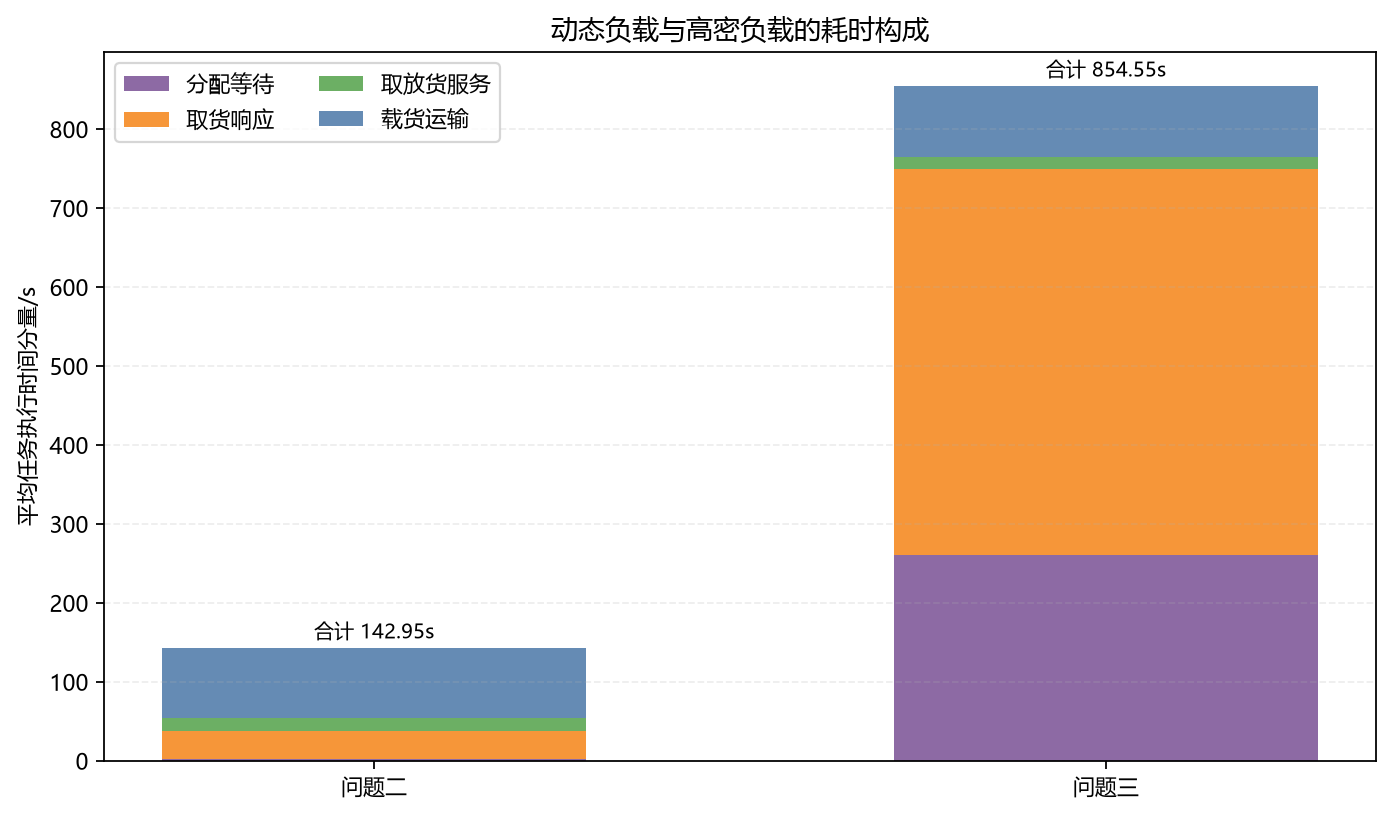
\includegraphics[width=0.88\textwidth]{time_components.png}
\caption{问题二、三任务执行时间分量对比}
\label{fig:time-components}
\end{figure}

图\ref{fig:priority-scatter}进一步按优先级展示问题三任务执行时间。散点的纵向离散说明，在严重超载下，释放时刻、Carrier 解锁、Source 位置和车辆可达性会共同影响单项时间，优先级不能完全抵消结构性排队；但高优先级任务由即时触发规则避免等待微批窗口，因而不会仅因批处理而额外滞后。该图用于解释调度效果，不据此宣称优先级与执行时间存在简单线性因果关系。

\begin{figure}[H]
\centering
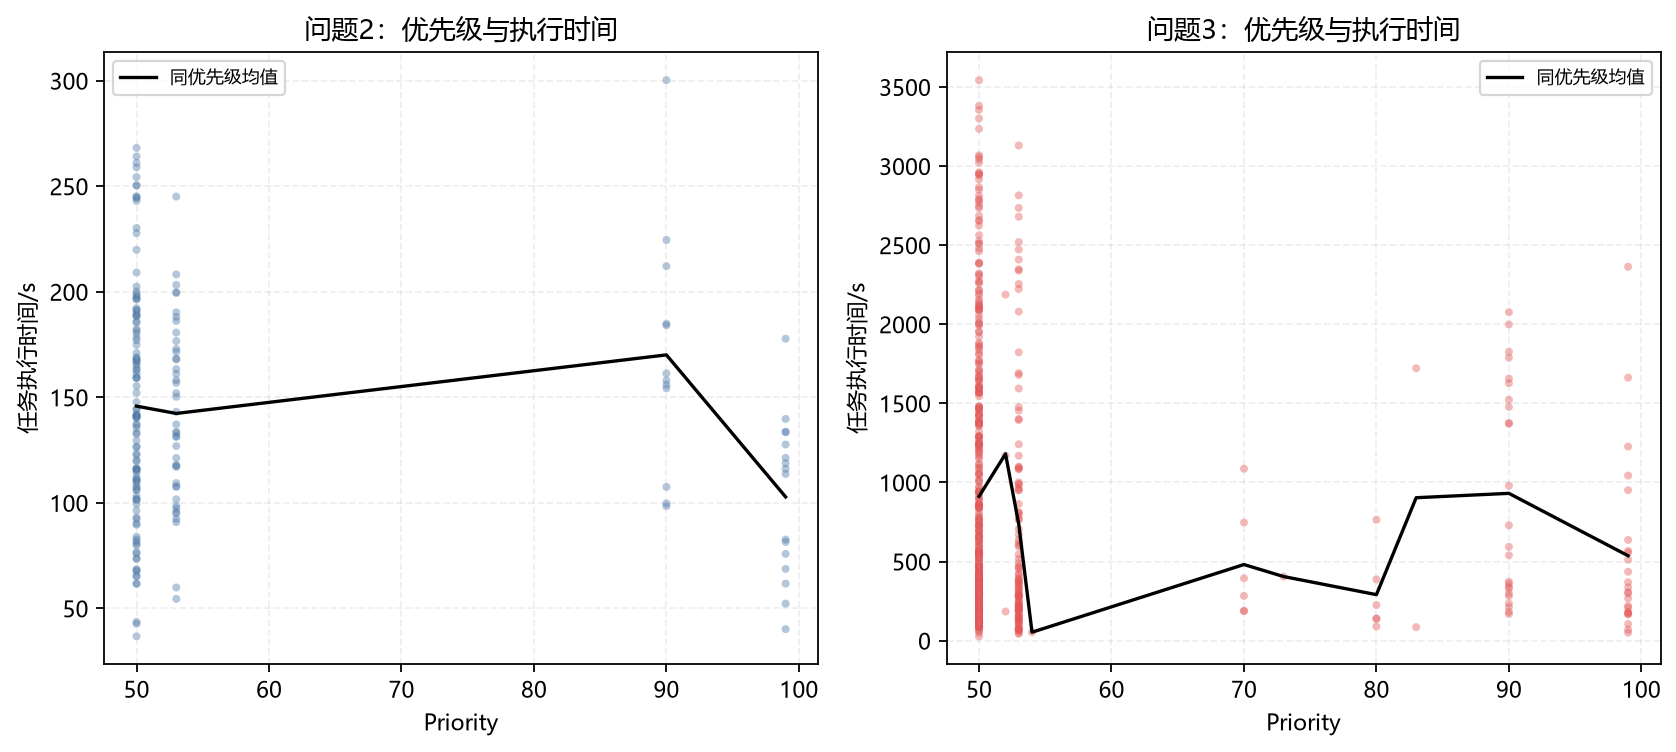
\includegraphics[width=0.88\textwidth]{priority_transfer_scatter.png}
\caption{问题三任务优先级与任务执行时间散点分布}
\label{fig:priority-scatter}
\end{figure}

问题二任务释放跨度约 $3558.816\ \mathrm{s}$，问题三仅约 $1797\ \mathrm{s}$，因此 Makespan 只增长 $9.33\%$ 不能说明高密性能接近；平均任务执行时间及其分解更能反映任务自身经历的排队延迟。

\section{模型验证与结果可信度}
\subsection{统一硬约束审计}

三问使用同一公共运动内核，代码哈希一致。正式轨迹和关键硬门见表\ref{tab:validation}。
\begin{table}[H]
\centering
\caption{三问正式轨迹与独立验证结果}
\renewcommand{\arraystretch}{1.35}
\begin{tabular*}{\textwidth}{@{\extracolsep{\fill}}lccc@{}}
\toprule[1pt]
项目 & 问题一 & 问题二 & 问题三\\ \midrule
完成任务 & 32/32 & 190/190 & 600/600\\
轨迹行数 & 33300 & 371540 & 406200\\
最大速度/(mm/s) & 710 & 710 & 710\\
最大加速度/(mm/s$^2$) & 2000 & 2000 & 2000\\
最小加速度/(mm/s$^2$) & -3000 & -3000 & -3000\\
程序内连续净空/mm & 325 & 325 & 325\\
独立保守净空下界/mm & 324.977513 & 324.977497 & 324.977470\\
硬违规数 & 0 & 0 & 0\\
\bottomrule[1pt]
\end{tabular*}
\label{tab:validation}
\end{table}

独立程序不导入求解器模块，而是从逐步轨迹按常加速度或“滑行--最大制动--静止”重建每个控制步，覆盖跨 Link 和拓扑切换。三问的保守净空下界均大于 $300\ \mathrm{mm}$，说明控制裕量能够吸收数值重建误差，且未依赖求解器内部变量自证安全。

验证采用由弱到强的四层证据链。第一层检查 CSV/工作簿字段、任务数和时间单调性；第二层检查每辆车的 Link 连续性、方向、速度和加速度；第三层检查 Port、MERGE、CurveGroup 容量以及 Carrier 前序；第四层从轨迹独立重建步内连续净空。只有前一层通过才进入后一层，任一层发现反例即保留车辆编号、时间区间、资源或车辆对并判候选不可行。

独立重建时，不直接信任输出的加速度字段，而由相邻速度反算
\begin{equation}
\hat a_k(t)=\frac{v_k(t+\Delta t)-v_k(t)}{\Delta t},
\end{equation}
再将其与 $[-3000,2000]$ 比较。若末速度为 0 且整步常减速度位移与记录位置不一致，则按式\eqref{eq:within-step-stop}识别“提前停稳”分段。该处理能区分合法的步内停车与非法的瞬时速度截断。

\subsection{在线信息隔离与输出一致性}

对问题二、三各选 3 个时间截点，将截点后所有未来任务的 Source、Destination、Priority、CarrierID 随机修改并反转任务顺序，再比较截点前的决策摘要。六组原始/扰动决策哈希完全一致，证明当前决策不依赖未来任务具体字段。

任务结果、逐步运行记录和算法指标同时导出 CSV 与附件 9 工作簿。验证器重新读取文件，检查每个 StepNo 恰有 20 辆车、QuestionNo 正确、时间字段单调、$C_j-r_j$ 与 TransferTime 一致、取放货各持续 $8\ \mathrm{s}$、Carrier 前序满足，并逐文件核对计算真源与答案目录的 SHA-256。

\subsection{安全裕量与误差传播分析}

控制器设置的理论车身净空为
\begin{equation}
g_{ctrl}=d_{ctrl}-L_v=1275-950=325\ \mathrm{mm},
\end{equation}
相对题设下限的名义裕量为 $25\ \mathrm{mm}$。独立重建得到的最小值略低于 325 mm，定义重建损失
\begin{equation}
\varepsilon_q=325-g_{min,q}^{ind}.
\end{equation}
三问分别为 $0.022487$、$0.022503$ 和 $0.022530\ \mathrm{mm}$，仅占 $25\ \mathrm{mm}$ 名义裕量的约 $0.09\%$。因此有效安全裕量仍分别为 $24.977513$、$24.977497$ 和 $24.977470\ \mathrm{mm}$。

\begin{table}[H]
\centering
\caption{连续净空裕量与可认证范围}
\label{tab:clearance-sensitivity}
\renewcommand{\arraystretch}{1.28}
\begin{tabular*}{\textwidth}{@{\extracolsep{\fill}}lrrrr@{}}
\toprule[1pt]
场景 & 控制目标/mm & 独立下界/mm & 相对 300 mm 裕量/mm & 可认证结论\\ \midrule
问题一 & 325 & 324.977513 & 24.977513 & 安全\\
问题二 & 325 & 324.977497 & 24.977497 & 安全\\
问题三 & 325 & 324.977470 & 24.977470 & 安全\\
问题三微批类 & 325 & 298 & $-2$ & 不安全，淘汰\\
\bottomrule[1pt]
\end{tabular*}
\end{table}

由表\ref{tab:clearance-sensitivity}可得一个不依赖再次仿真的灵敏度结论：若题设最小净空提高到不超过 $324.977470\ \mathrm{mm}$，三问现有正式轨迹仍可由当前证据认证；若要求继续提高，则必须重新增大 $d_{ctrl}$ 并仿真，不能外推。反之，三个问题三微批候选在现行 $300\ \mathrm{mm}$ 下已经不足，更不可能通过更严格标准。

关键输入误差的传播路径见表\ref{tab:error-propagation}。其中 P17 的位置修订在构图前覆盖，避免错误 Port 偏移进入全部 OD 距离；车辆长度和净空下限直接进入式\eqref{eq:reference-gap}，属于最敏感参数；Link 长度和限速影响预计时间，但正式轨迹仍会受到资源与运动控制二次校验。

\begin{table}[H]
\centering
\caption{关键数据误差的影响路径与控制措施}
\label{tab:error-propagation}
\renewcommand{\arraystretch}{1.28}
\begin{tabular*}{\textwidth}{@{\extracolsep{\fill}}p{2.7cm}p{4.4cm}p{4.2cm}p{2.4cm}@{}}
\toprule[1pt]
输入或参数 & 可能传播后果 & 本文控制措施 & 剩余风险\\ \midrule
Port 所在 Link/offset & OD 距离、服务停车点和路径全部偏移 & 构图前强制覆盖 P17 修订并审计可达性 & 低\\
Link 长度与方向 & 最短路、前后车有向距离错误 & 逐 Link 连续性和禁止逆行检查 & 低\\
车辆长度 $L_v$ & 参考点距离到车身净空换算错误 & 统一使用式\eqref{eq:reference-gap}并独立重建 & 极低\\
控制步长 $\Delta t$ & 端点采样可能漏掉步内最小净空 & 分段解析极值而非仅查离散点 & 低\\
代理目标权重 & 改变搜索路径并可能陷入局部最优 & 只用于候选排序，正式目标重新仿真 & 中\\
\bottomrule[1pt]
\end{tabular*}
\end{table}

\subsection{结果可重复性与边界}

问题一固定随机种子 20260815、迭代 1200 轮；问题二、三使用确定性平局规则。对同一输入重复运行时，任务链、轨迹摘要和指标文件哈希一致。需要强调的是，该重复性结论针对当前附件、控制步长、巡航上限和资源定义；若修改 Link 封闭状态、车辆数量、服务时间或最小净空，应重新执行完整硬门，不应只替换结果表中的参数。

\section{模型评价与改进}
\subsection{模型优点}
\begin{enumerate}
\item 分层结构兼顾优化与物理可行，高层算法可替换，底层统一保证方向、运动学、跟驰和资源约束。
\item 模型选择有对照依据：问题一比较三种静态算法，问题二比较四类在线策略，问题三明确淘汰三个更快但不安全的候选。
\item 连续安全证据完整：从净空口径化简、制动速度控制到独立分段轨迹回放形成三层验证。
\item 在线性通过反事实测试，而非只依赖程序自报的未来泄漏计数。
\item 负载分解表明高密瓶颈来自车辆供给、Carrier 解锁与 Source 排队，为系统扩容提供依据。
\end{enumerate}

\subsection{局限与改进}
\begin{enumerate}
\item 正式控制采用 $710\ \mathrm{mm/s}$ 保守巡航上限，未充分利用限速为 1000 或 $3000\ \mathrm{mm/s}$ 的 Link，所得为可行优化解而非全局最优。
\item 问题一 ALNS 只在固定种子和 1200 轮预算下运行，尚缺少多随机种子置信区间。
\item 问题二 balanced 与基线同分，当前报价权重尚未在该数据集上产生可辨识增益。
\item 问题三压力与时隙候选在汇流拓扑切换处失效，高层预约必须与低层新邻接连续安全联合设计。
\item 当前未考虑设备故障、Link 临时封闭和服务时间随机波动。
\end{enumerate}

后续可用模型预测控制动态开放高速 Link，在保持式\eqref{eq:safe-speed}和式\eqref{eq:stop-speed}可行的前提下提高巡航速度；对 ALNS 做多种子并行；在高密场景中把 MERGE 的空间接纳条件直接写入时隙生成，要求车辆进入下游后仍满足 $1275\ \mathrm{mm}$ 参考间距；进一步可建立随机到达下的鲁棒滚动时域模型。

\section{结论}

本文建立了适用于三类负载场景的 OHT 分层协同调度模型。统一路网层保留 Port 的 Link 内实际位置，统一交通层用参考点距离、制动速度上界和分段轨迹极值保证任意时刻安全，上层则根据任务信息模式分别采用静态 ALNS 和在线滚动拍卖。

问题一中，ALNS 将 32 项静态任务平均执行时间降至 $171.39375\ \mathrm{s}$，较基准下降 $17.01\%$。问题二中，负载均衡滚动拍卖在线完成 190 项任务，平均执行时间为 $142.946305\ \mathrm{s}$，反事实检验未发现未来信息泄漏。问题三中，直接滚动方案是四个高密候选中唯一通过连续净空硬门的方案，600 项任务平均执行时间为 $854.551420\ \mathrm{s}$。高密场景的载货运输时间基本不变，但分配等待和取货响应大幅增加，说明系统瓶颈已从路径长度转移到车辆供给、Carrier 解锁和 Source 侧排队。

三问正式轨迹均完成全部任务，速度、加减速度、Port/MERGE/Curve 容量、Carrier 前序和在线信息约束全部通过；独立连续净空保守下界分别为 $324.977513$、$324.977497$ 和 $324.977470\ \mathrm{mm}$，高于题目规定的 $300\ \mathrm{mm}$。因此，所给方案是在当前巡航速度与离散控制参数下可复核、可复现的安全优化方案。

\section*{AI 工具使用与引用声明}

本文在论文撰写与排版阶段使用 OpenAI Codex（GPT-5 系列）辅助完成长篇 LaTeX 结构整理、既有模型说明的语言润色、公式符号一致性检查、图表代码生成建议及编译错误排查\cite{openai2026}。AI 工具未替代参赛队员进行赛题决策：模型路线、算法选择、参数取值、正式候选筛选以及所有结论均由参赛队员结合题目附件和本地程序输出审定。文中三问数值均来自本地可重复运行的求解与仿真文件，并经过任务结果复算、轨迹硬约束审计和独立连续净空重建；对于 AI 生成或改写的文字、公式解释和图表标题，参赛队员逐项核对后决定采用、修改或删除。本文对最终内容、数据真实性和学术规范承担全部责任。

\begin{thebibliography}{99}
\bibitem{ropke2006} Ropke S, Pisinger D. An adaptive large neighborhood search heuristic for the pickup and delivery problem with time windows[J]. Transportation Science, 2006, 40(4): 455--472.
\bibitem{shaw1998} Shaw P. Using constraint programming and local search methods to solve vehicle routing problems[C]//Principles and Practice of Constraint Programming. Berlin: Springer, 1998: 417--431.
\bibitem{bertsekas1988} Bertsekas D P. The auction algorithm: A distributed relaxation method for the assignment problem[J]. Annals of Operations Research, 1988, 14: 105--123.
\bibitem{kirkpatrick1983} Kirkpatrick S, Gelatt C D, Vecchi M P. Optimization by simulated annealing[J]. Science, 1983, 220(4598): 671--680.
\bibitem{rawlings2017} Rawlings J B, Mayne D Q, Diehl M. Model Predictive Control: Theory, Computation, and Design[M]. 2nd ed. Madison: Nob Hill Publishing, 2017.
\bibitem{sutton2018} Sutton R S, Barto A G. Reinforcement Learning: An Introduction[M]. 2nd ed. Cambridge: MIT Press, 2018.
\bibitem{openai2026} OpenAI. Codex: AI coding and writing assistant based on the GPT-5 series[EB/OL]. San Francisco: OpenAI, 2026.
\end{thebibliography}

\newpage
\appendix
\section*{附录 A：正式输出文件}

问题一正式结果位于 \verb|outputs/q1|，问题二位于 \verb|outputs/q2|，问题三位于 \verb|outputs/q3|。每个目录均包含附件 9 工作簿、任务结果 CSV、完整 OHT 逐步轨迹、算法评价指标、方案配置和约束审计；三问答案目录已与计算真源逐文件哈希同步。

\section*{附录 B：核心求解伪代码}

\noindent\textbf{静态 ALNS：}
\begin{enumerate}
\item 用全局增量插入生成 20 条初始任务链；
\item 按自适应权重选择破坏算子并移除若干任务；
\item 用 regret-3 在全部车辆、全部位置中修复；
\item 计算代理目标，以模拟退火准则接受；
\item 记录历史最好解，重复 1200 轮；
\item 对最好任务链运行完整物理仿真，通过硬门后输出。
\end{enumerate}

\noindent\textbf{在线滚动拍卖：}
\begin{enumerate}
\item 在事件时刻更新已释放任务，并按 Carrier 前序生成 $J^V(t)$；
\item 对每个任务、车辆和插入位置计算报价；
\item 提交最小报价并更新车辆承诺队列，直至 $J^V(t)$ 为空；
\item 在 $0.2\ \mathrm{s}$ 仿真中执行任务、仲裁资源并更新位置；
\item 新事件到达后返回第 1 步，直到全部任务完成。
\end{enumerate}

\section*{附录 C：AI 辅助内容的人工复核清单}

\begin{enumerate}
\item 对所有由 AI 辅助整理的公式，逐项核对变量是否在正文首次出现处定义，单位是否一致，等号变形是否保持方向与定义域；
\item 对所有表格数值，与 \verb|outputs/q1|、\verb|outputs/q2|、\verb|outputs/q3| 及正式复核汇总文件交叉核验；
\item 对算法比较中的备选方法，只陈述其一般适用性和本题不采用理由，不虚构未实际运行的数值结果；
\item 对问题三三个不安全候选保留 $298\ \mathrm{mm}$ 反例，禁止把其较小平均时间表述为有效改进；
\item 最终 PDF 由 XeLaTeX 本地编译，并对摘要、公式、图表、页码、目录和参考文献进行逐页检查。
\end{enumerate}

\end{document}
